\section{系统测试与分析}\label{chap:testing}

本章介绍系统的测试环境、功能测试、隐写性能分析以及跨平台兼容性测试的过程与结果。

\subsection{测试环境}

系统测试所使用的软硬件环境如\cref{tab:test_env}所示。

\begin{table}[htbp]
    \caption{测试环境配置}
    \centering
    \begin{tabular}{ll}
        \hline
        \textbf{项目} & \textbf{配置} \\
        \hline
        操作系统 & Ubuntu 22.04 LTS (WSL2) \\
        CPU & Intel Core i7-12700H（笔记本） \\
        GPU & NVIDIA GeForce RTX 3060 Laptop（6\,GB，CUDA 12.x） \\
        内存 & 16 GB \\
        Python 版本 & 3.10+（Sage 环境） \\
        Android 测试设备 & Android 12+ 物理设备/模拟器 \\
        Web 浏览器 & Google Chrome 120+ \\
        Node.js 版本 & 18+ \\
        \hline
    \end{tabular}
    \label{tab:test_env}
\end{table}

服务端运行在本地开发环境中，使用 \texttt{uvicorn} 作为 ASGI 服务器，监听 8000 端口。Pulsar 和 SparSamp 算法在 Sage 数学软件环境中运行，使用 CUDA 加速扩散模型的推理计算。

\subsection{功能测试}

\subsubsection{用户注册与登录测试}

测试了用户注册和登录的正常流程与异常处理，测试用例及结果如\cref{tab:test_auth}所示。

\begin{table}[htbp]
    \caption{用户注册与登录测试用例}
    \centering
    \begin{tabular}{clc}
        \hline
        \textbf{编号} & \textbf{测试内容} & \textbf{结果} \\
        \hline
        T-01 & 正常注册新用户 & 通过 \\
        T-02 & 注册已存在的用户名 & 通过（正确提示错误） \\
        T-03 & 注册时用户名格式校验（过短/特殊字符） & 通过 \\
        T-04 & 注册时密码长度校验（少于6字符） & 通过 \\
        T-05 & 正确用户名密码登录 & 通过 \\
        T-06 & 错误密码登录 & 通过（正确提示错误） \\
        T-07 & 登录后获取用户信息 & 通过 \\
        T-08 & 注册后自动生成邀请码 & 通过 \\
        T-09 & 登录令牌有效性验证（/auth/me） & 通过 \\
        T-10 & 令牌过期后的请求拒绝 & 通过（401 响应） \\
        \hline
    \end{tabular}
    \label{tab:test_auth}
\end{table}

用户注册和登录后的界面效果如\cref{fig:ch5_register}所示。

\begin{figure}[htbp]
    \centering
    \begin{subfigure}[b]{0.38\textwidth}
        \centering
        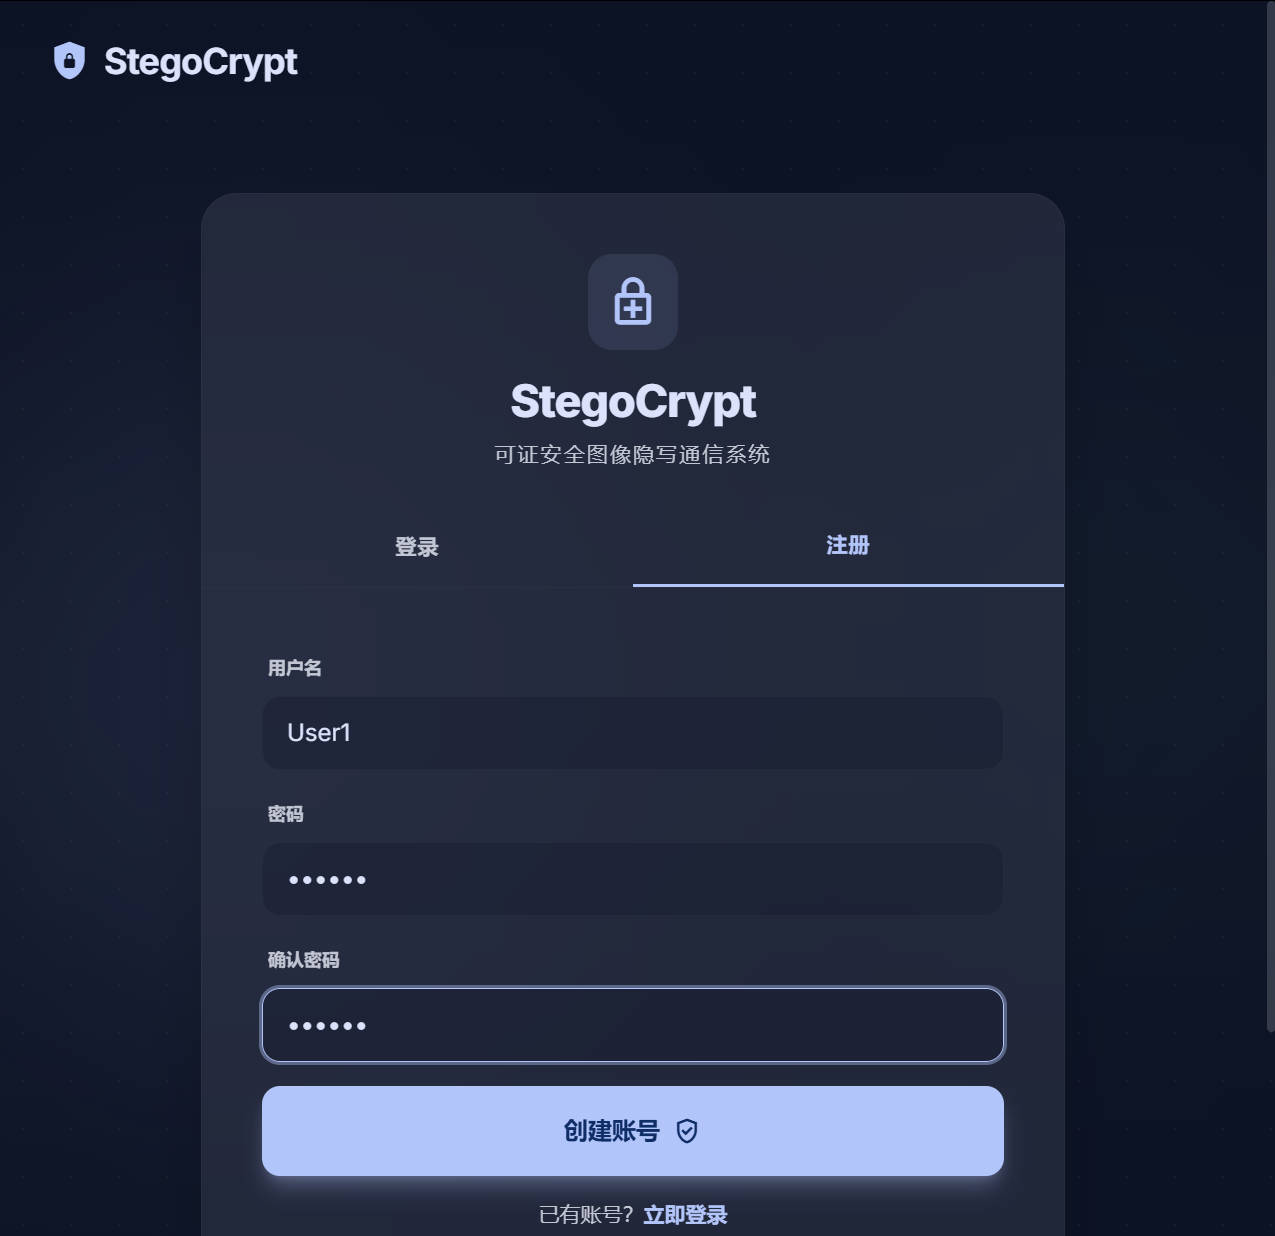
\includegraphics[width=\textwidth]{img/ch5_01_register.jpg}
        \caption{Web 端注册页面}
        \label{fig:ch5_register_web}
    \end{subfigure}
    \hfill
    \begin{subfigure}[b]{0.38\textwidth}
        \centering
        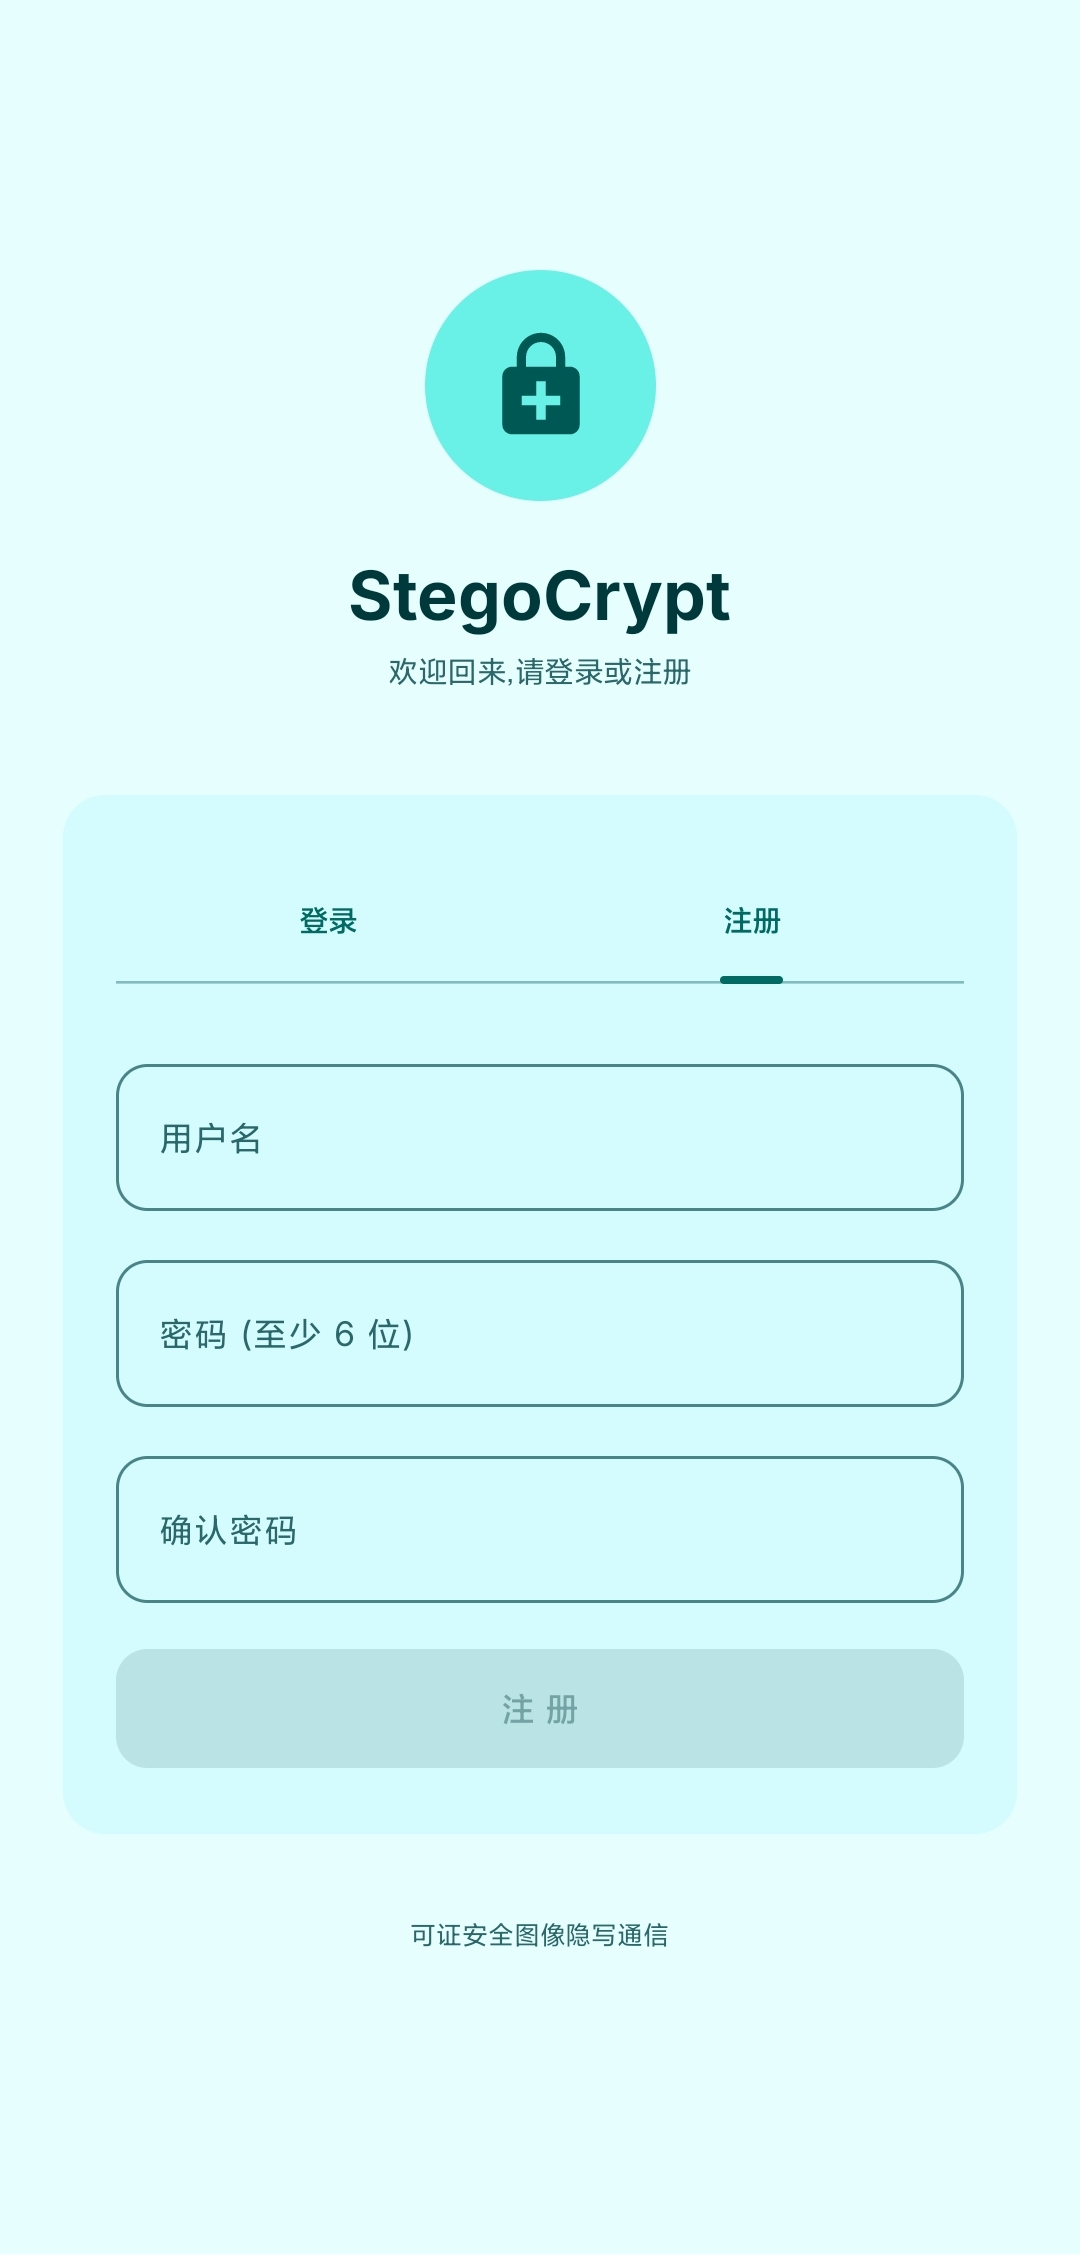
\includegraphics[height=6cm]{img/ch5_01_register_phone.jpg}
        \caption{Android 端注册页面}
        \label{fig:ch5_register_android}
    \end{subfigure}

    \vspace{0.5em}
    \begin{subfigure}[b]{0.55\textwidth}
        \centering
        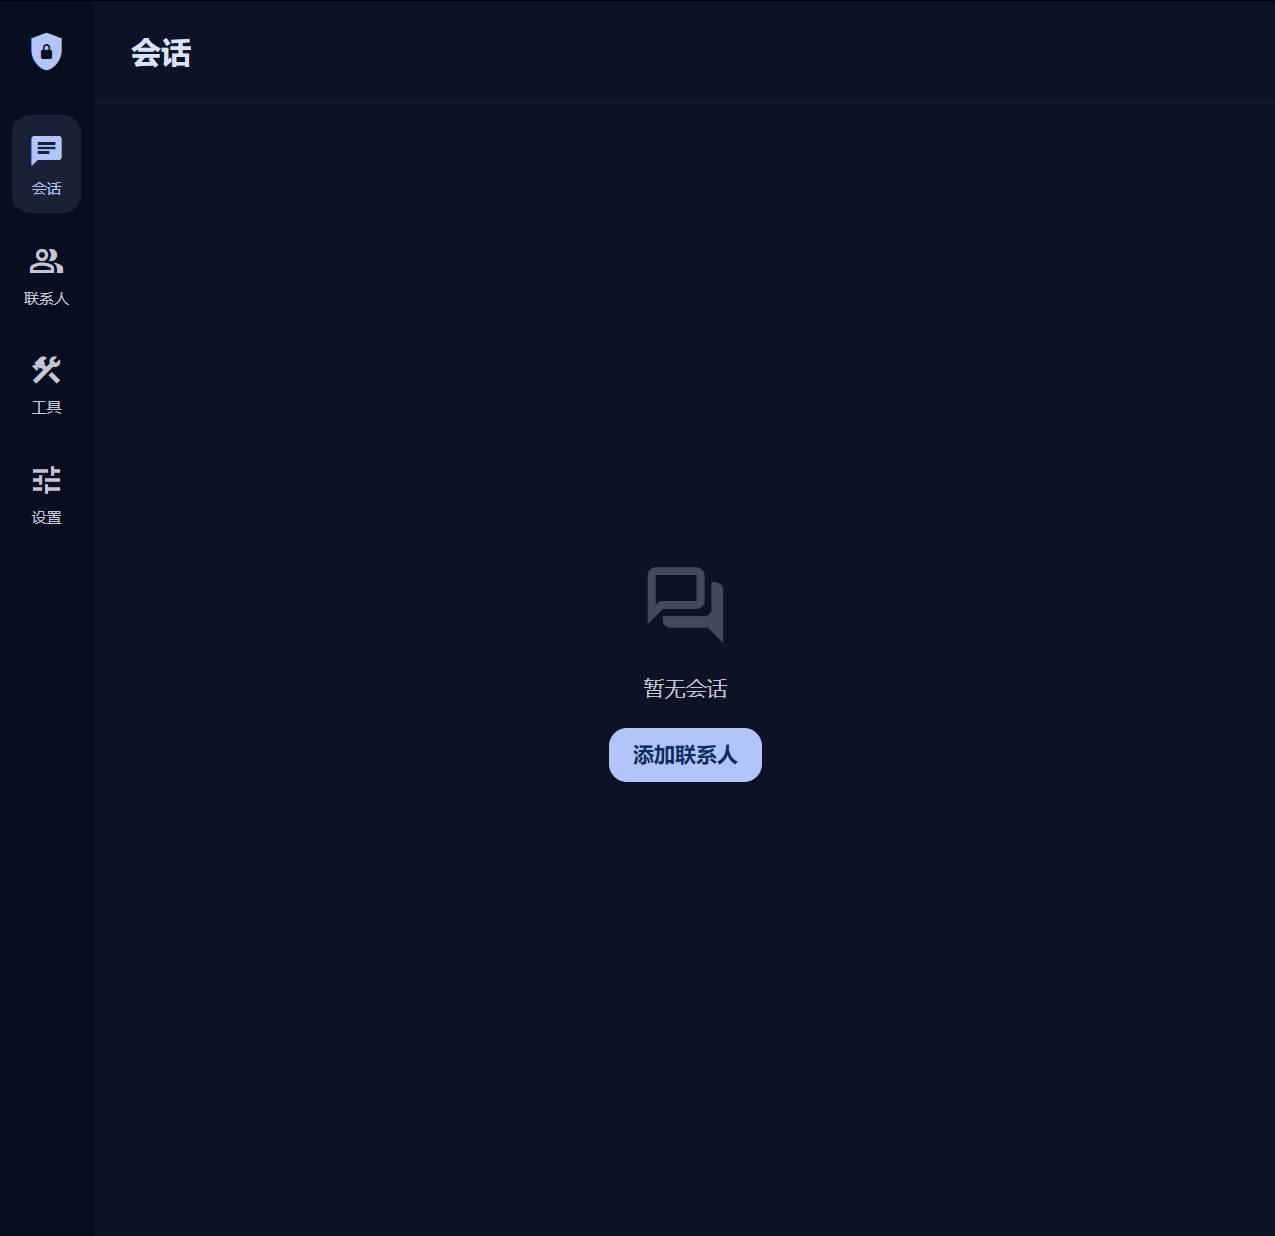
\includegraphics[width=\textwidth]{img/ch5_02_home.jpg}
        \caption{登录后主页}
        \label{fig:ch5_home}
    \end{subfigure}
    \caption{用户注册与登录界面}
    \label{fig:ch5_register}
\end{figure}

\subsubsection{好友管理测试}

测试了好友添加的完整流程，包括邀请码查询、好友请求发送与处理等，测试用例及结果如\cref{tab:test_friend}所示。

\begin{table}[htbp]
    \caption{好友管理测试用例}
    \centering
    \begin{tabular}{clc}
        \hline
        \textbf{编号} & \textbf{测试内容} & \textbf{结果} \\
        \hline
        T-11 & 通过邀请码查找用户 & 通过 \\
        T-12 & 发送好友请求（对方在线） & 通过 \\
        T-13 & 发送好友请求（对方离线） & 通过（离线缓存生效） \\
        T-14 & 接受好友请求 & 通过 \\
        T-15 & 拒绝好友请求 & 通过 \\
        T-16 & 屏蔽用户 & 通过（后续消息被过滤） \\
        T-17 & 重复发送好友请求（去重） & 通过 \\
        T-18 & 重置邀请码 & 通过（旧码失效） \\
        T-19 & 好友请求计数显示 & 通过 \\
        \hline
    \end{tabular}
    \label{tab:test_friend}
\end{table}

好友管理的界面效果如\cref{fig:ch5_friend}所示。

\begin{figure}[htbp]
    \centering
    \begin{subfigure}[b]{0.35\textwidth}
        \centering
        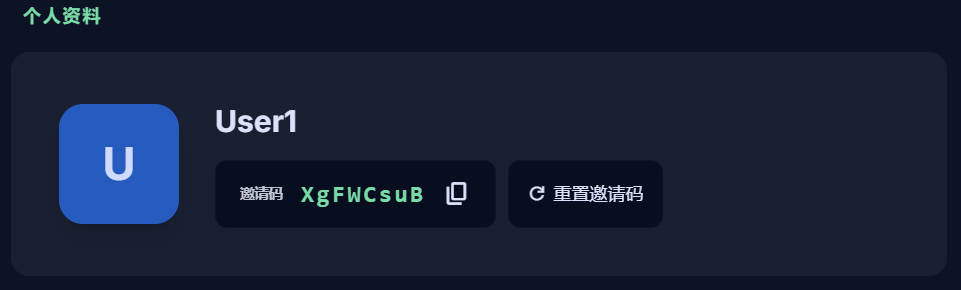
\includegraphics[width=\textwidth]{img/ch5_03_invitecode.jpg}
        \caption{邀请码页面}
        \label{fig:ch5_invitecode}
    \end{subfigure}
    \hfill
    \begin{subfigure}[b]{0.28\textwidth}
        \centering
        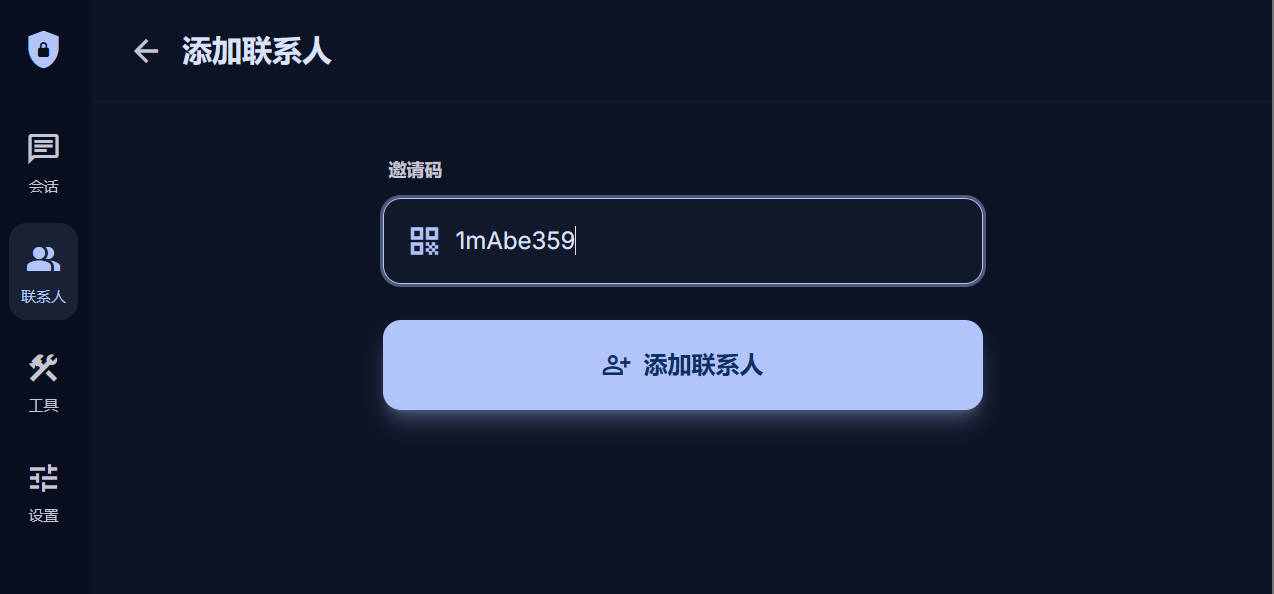
\includegraphics[width=\textwidth]{img/ch5_04_friend_request.jpg}
        \caption{Web 端好友请求}
        \label{fig:ch5_friend_web}
    \end{subfigure}
    \hfill
    \begin{subfigure}[b]{0.28\textwidth}
        \centering
        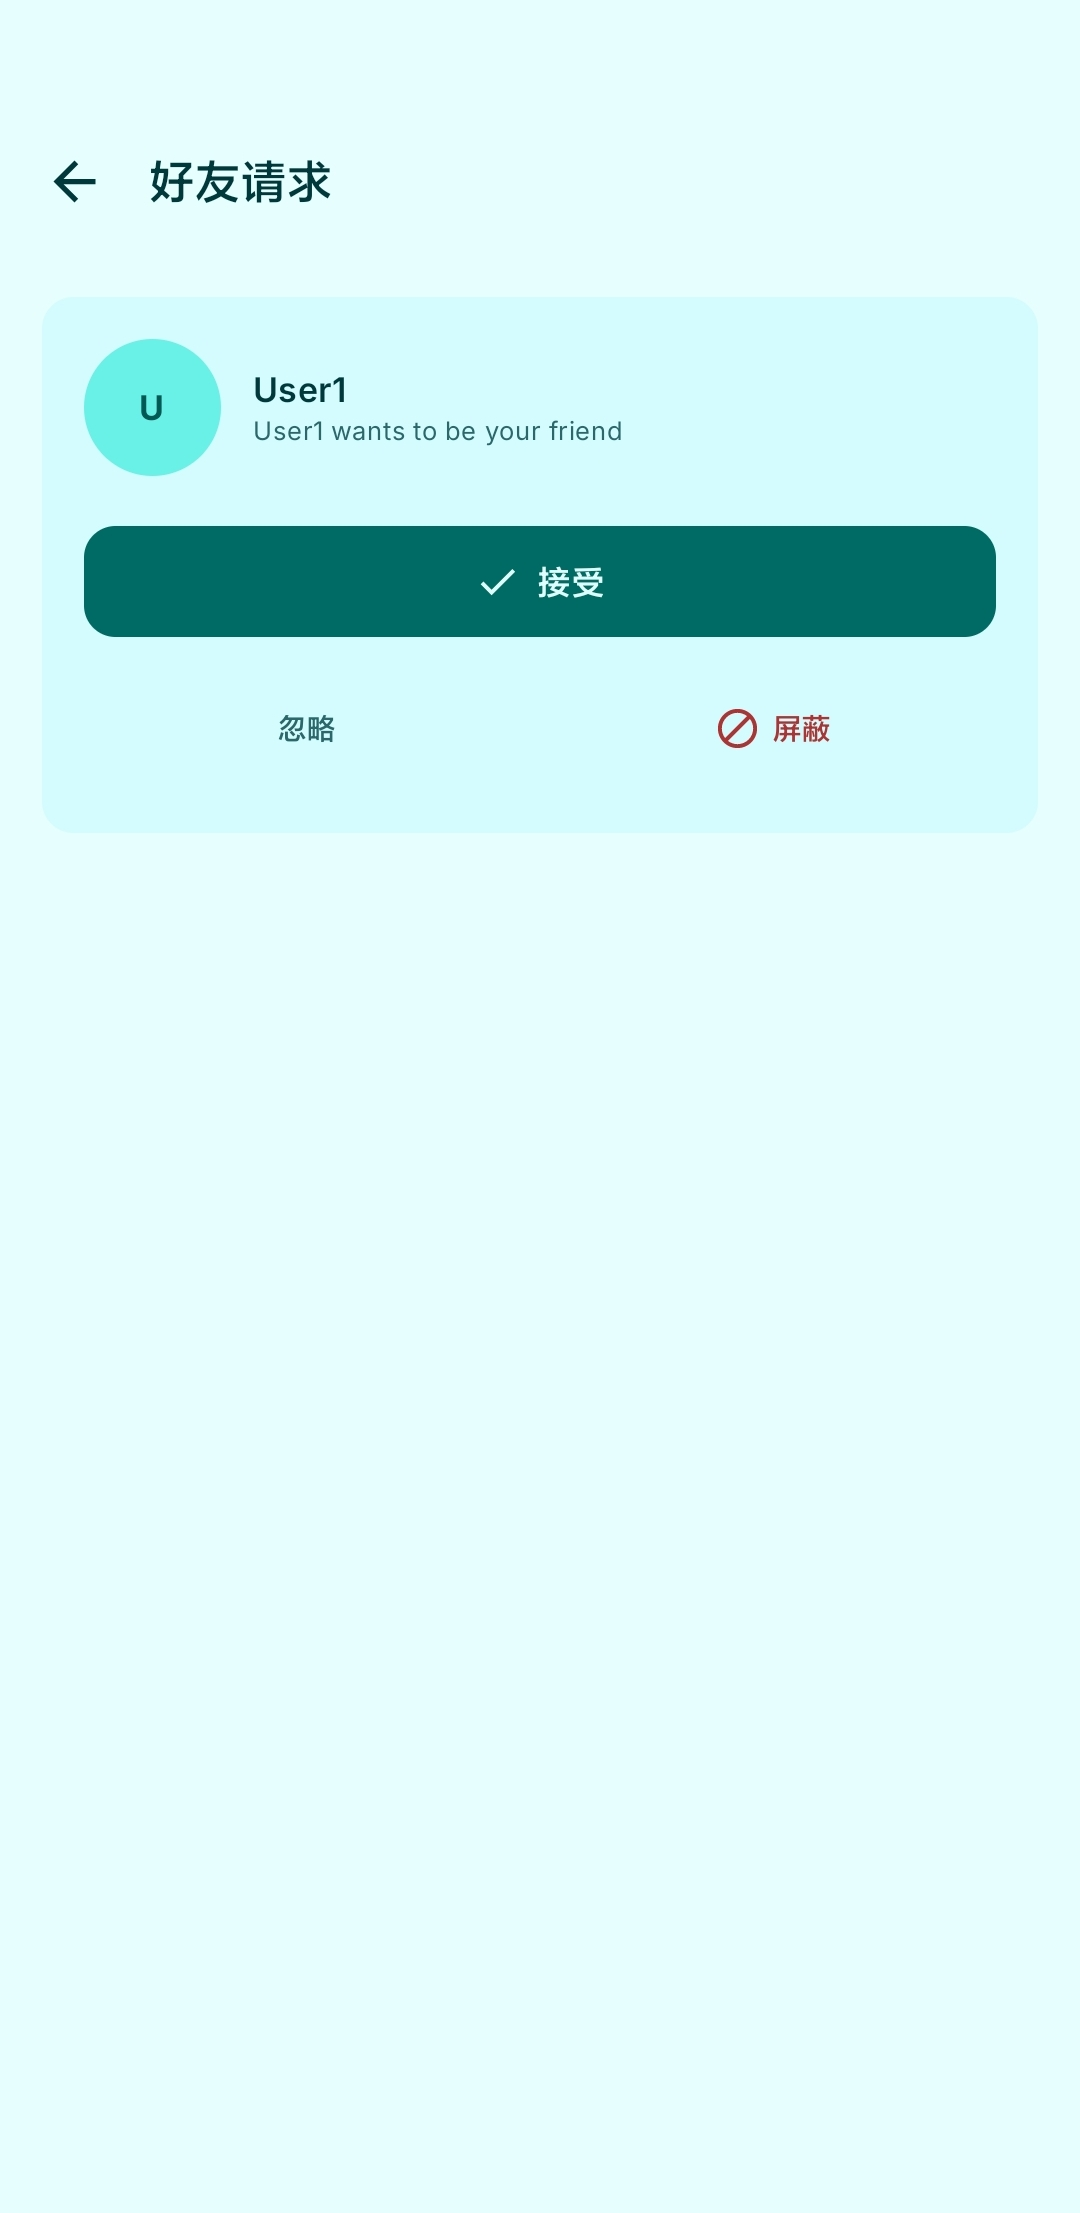
\includegraphics[height=6cm]{img/ch5_04_friend_request_phone.jpg}
        \caption{Android 端好友请求}
        \label{fig:ch5_friend_android}
    \end{subfigure}
    \caption{好友管理界面}
    \label{fig:ch5_friend}
\end{figure}

\subsubsection{消息收发与生命周期测试}

测试了普通消息和隐写消息在不同场景下的收发功能，以及消息状态管理，测试用例及结果如\cref{tab:test_msg}所示。

\begin{table}[htbp]
    \caption{消息收发与生命周期测试用例}
    \centering
    \begin{tabular}{clc}
        \hline
        \textbf{编号} & \textbf{测试内容} & \textbf{结果} \\
        \hline
        T-20 & 发送普通文本消息（双方在线） & 通过 \\
        T-21 & 发送普通文本消息（对方离线后上线） & 通过 \\
        T-22 & 消息状态：sending $\to$ sent（ack） & 通过 \\
        T-23 & 消息状态：sent $\to$ delivered（回执） & 通过 \\
        T-24 & 消息状态：delivered $\to$ read（回执） & 通过 \\
        T-25 & 发送隐写消息（嵌入与传输） & 通过 \\
        T-26 & 接收隐写消息并提取文本 & 通过 \\
        T-27 & 消息本地持久化存储 & 通过 \\
        T-28 & 隐写图像保存到本地 & 通过 \\
        \hline
    \end{tabular}
    \label{tab:test_msg}
\end{table}

消息收发的界面效果如\cref{fig:ch5_chat}所示。

\begin{figure}[htbp]
    \centering
    \begin{subfigure}[b]{0.38\textwidth}
        \centering
        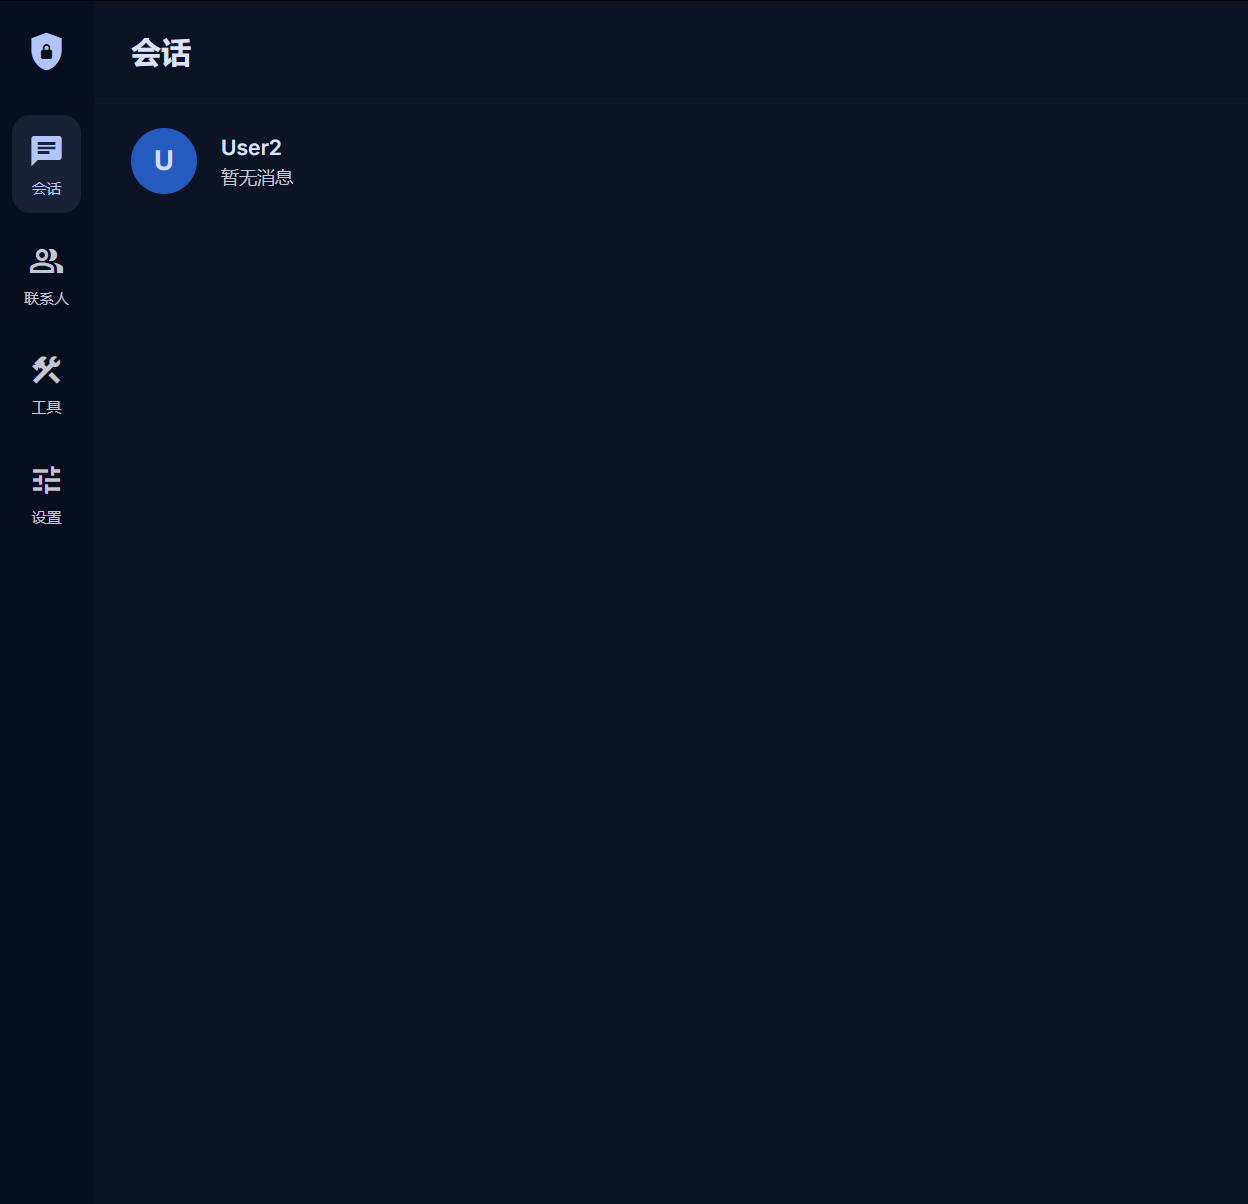
\includegraphics[width=\textwidth]{img/ch5_06_chat_list.jpg}
        \caption{Web 端聊天列表}
        \label{fig:ch5_chatlist_web}
    \end{subfigure}
    \hfill
    \begin{subfigure}[b]{0.38\textwidth}
        \centering
        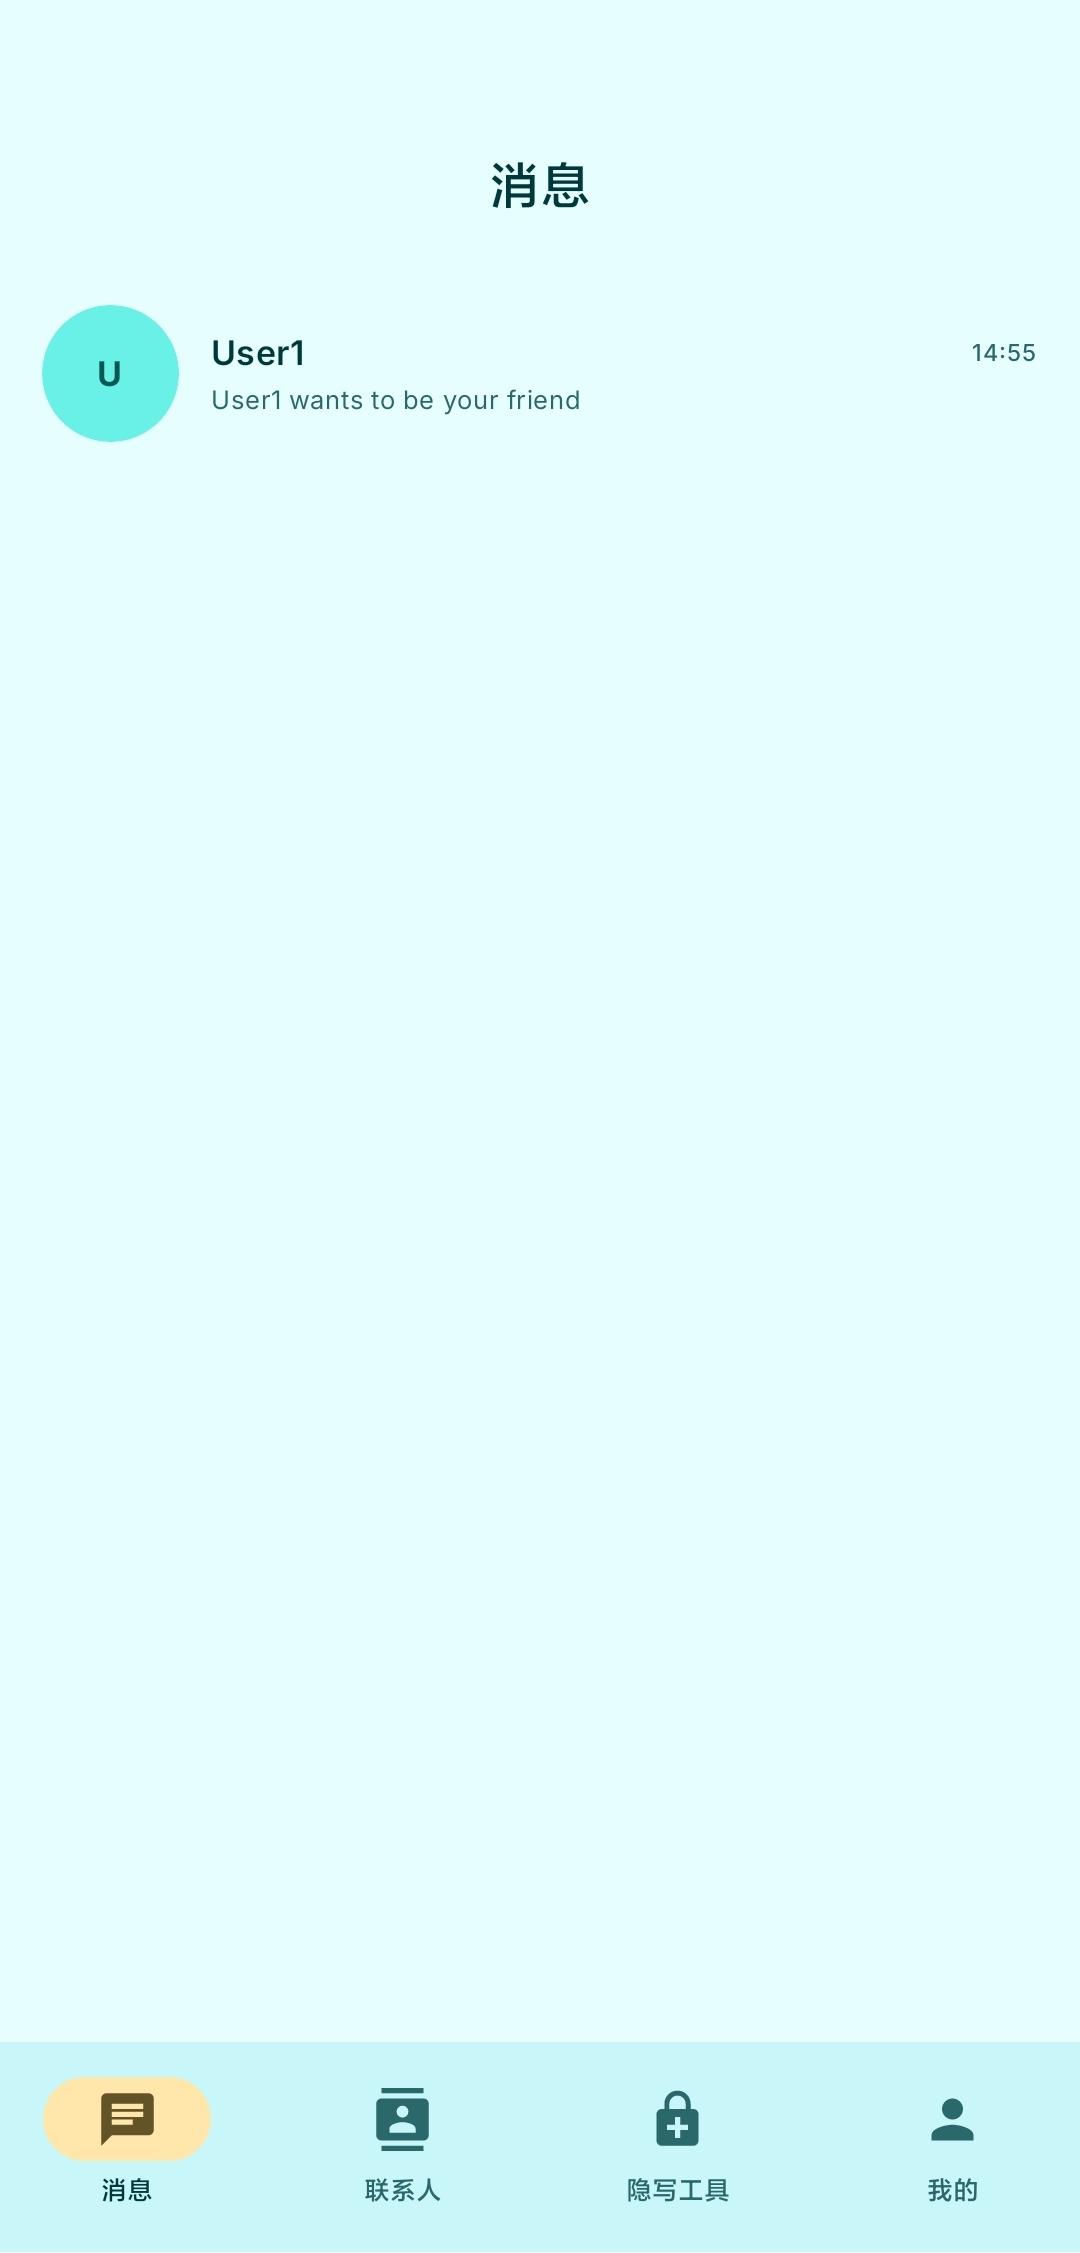
\includegraphics[height=5.5cm]{img/ch5_06_chat_list_phone.jpg}
        \caption{Android 端聊天列表}
        \label{fig:ch5_chatlist_android}
    \end{subfigure}

    \vspace{0.5em}
    \begin{subfigure}[b]{0.38\textwidth}
        \centering
        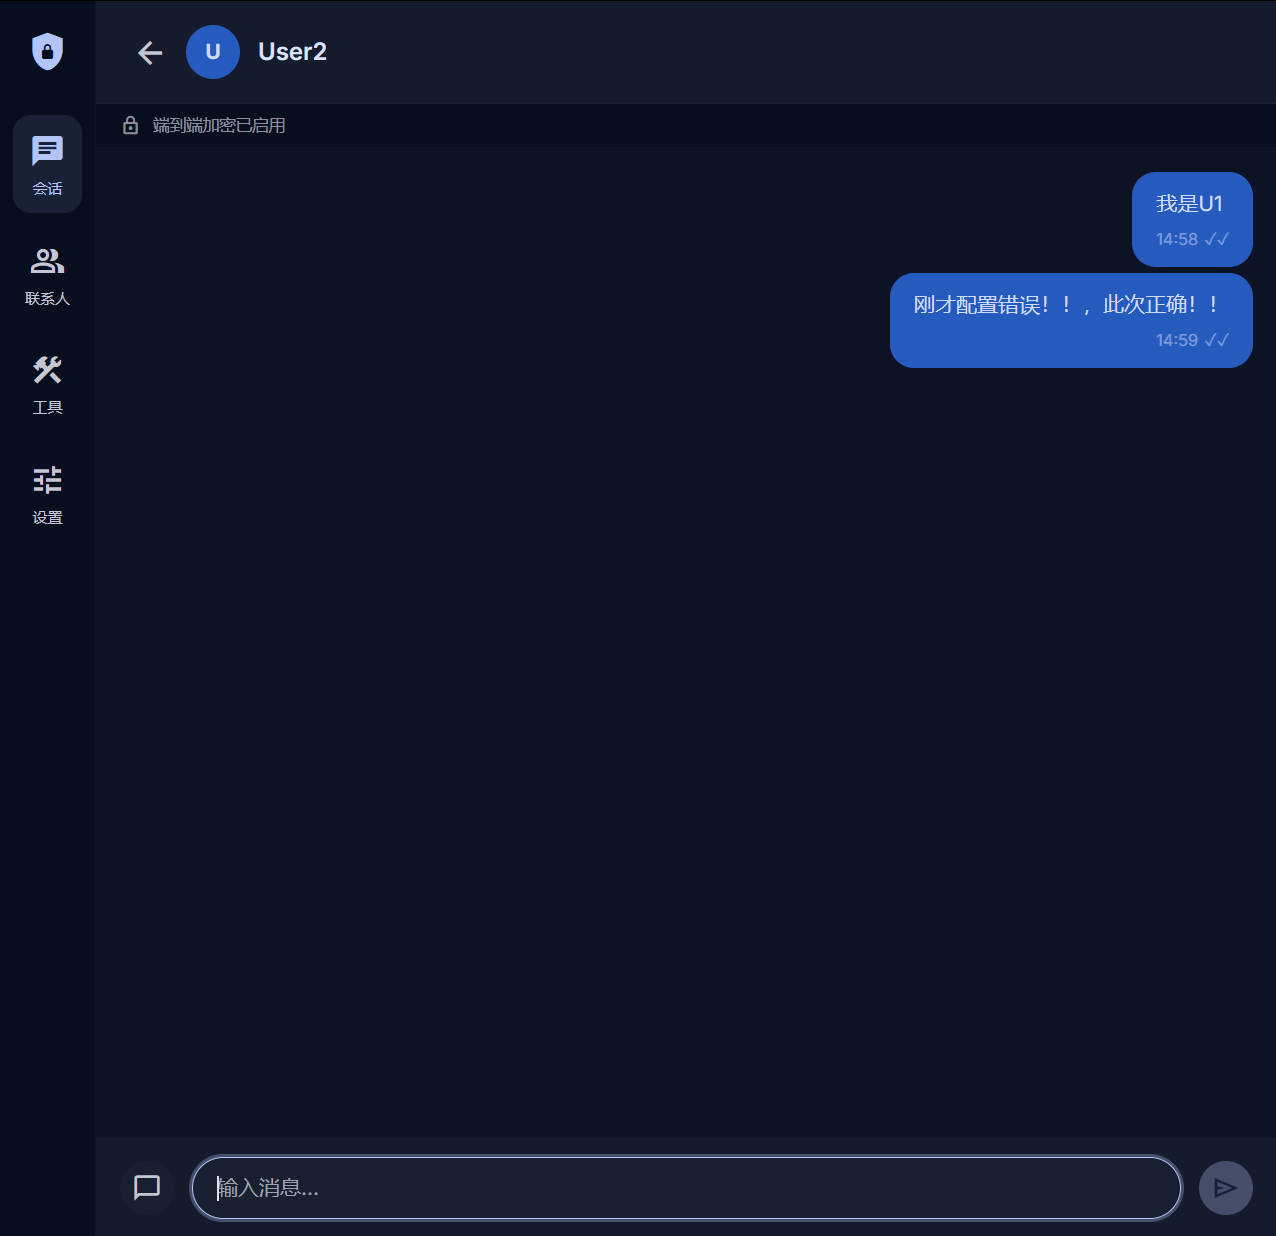
\includegraphics[width=\textwidth]{img/ch5_07_normal_chat.jpg}
        \caption{Web 端普通消息}
        \label{fig:ch5_normal_web}
    \end{subfigure}
    \hfill
    \begin{subfigure}[b]{0.38\textwidth}
        \centering
        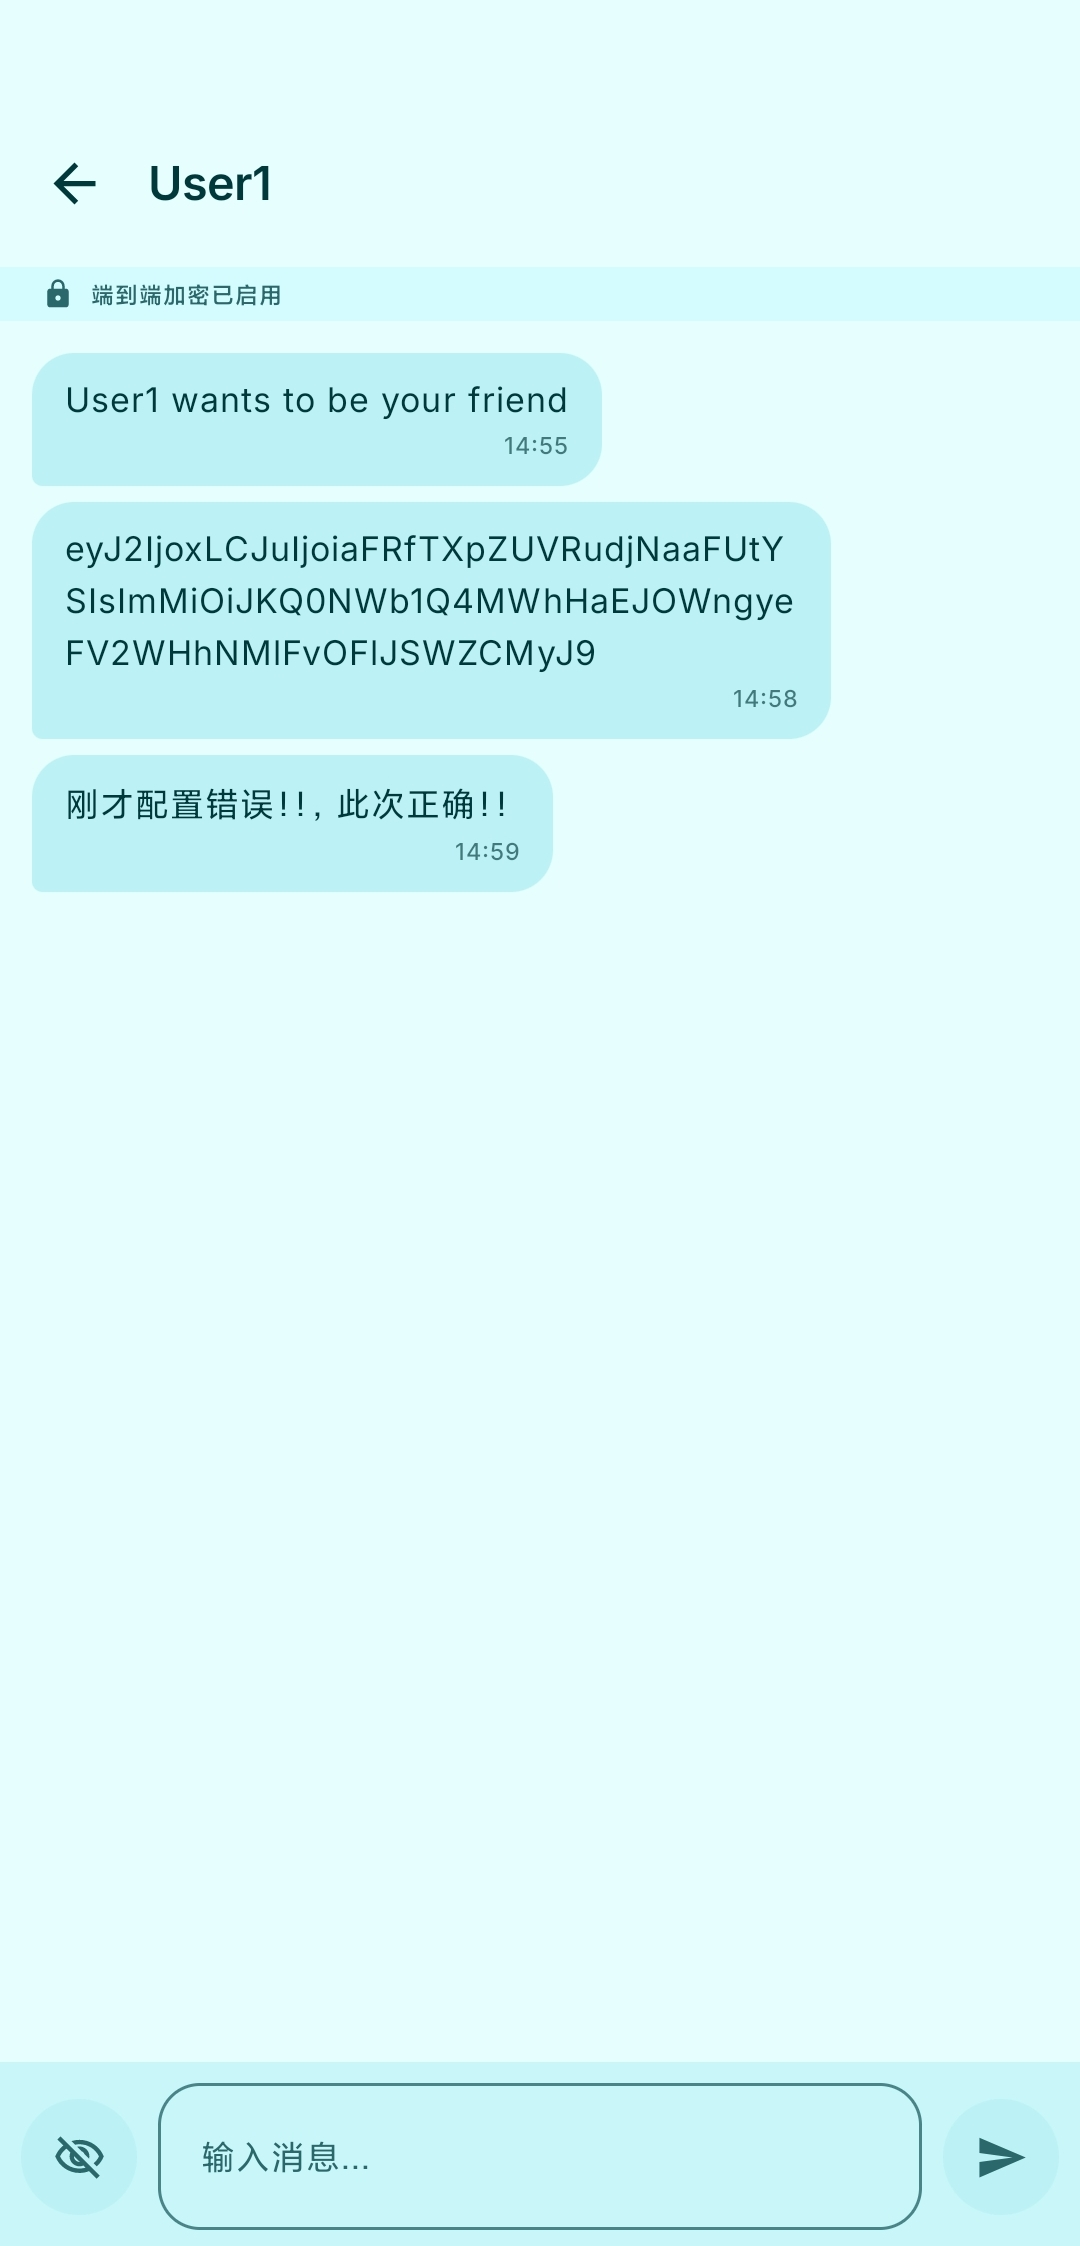
\includegraphics[height=5.5cm]{img/ch5_07_normal_chat_phone.jpg}
        \caption{Android 端普通消息}
        \label{fig:ch5_normal_android}
    \end{subfigure}
    \caption{消息收发界面}
    \label{fig:ch5_chat}
\end{figure}

\subsubsection{端到端加密测试}

测试了端到端加密的密钥派生、消息加解密和跨平台兼容性，测试用例及结果如\cref{tab:test_e2ee}所示。

\begin{table}[htbp]
    \caption{端到端加密测试用例}
    \centering
    \begin{tabular}{clc}
        \hline
        \textbf{编号} & \textbf{测试内容} & \textbf{结果} \\
        \hline
        T-29 & 助记词保存与指纹生成 & 通过 \\
        T-30 & 用户密钥派生一致性（相同助记词） & 通过 \\
        T-31 & 消息密钥对称性（deriveMkey(A,B) = deriveMkey(B,A)） & 通过 \\
        T-32 & 消息加密与解密（SealedMessage round-trip） & 通过 \\
        T-33 & 错误密钥解密失败（返回 null） & 通过 \\
        T-34 & 未加密消息兼容处理（legacy plaintext） & 通过 \\
        T-35 & E2EE 状态横幅显示（三种状态） & 通过 \\
        T-36 & 指纹对比验证（双方一致） & 通过 \\
        T-37 & Android 加密 $\to$ Web 解密（跨平台） & 通过 \\
        T-38 & Web 加密 $\to$ Android 解密（跨平台） & 通过 \\
        \hline
    \end{tabular}
    \label{tab:test_e2ee}
\end{table}

端到端加密的界面效果如\cref{fig:ch5_e2ee}所示。

\begin{figure}[htbp]
    \centering
    \begin{subfigure}[b]{0.45\textwidth}
        \centering
        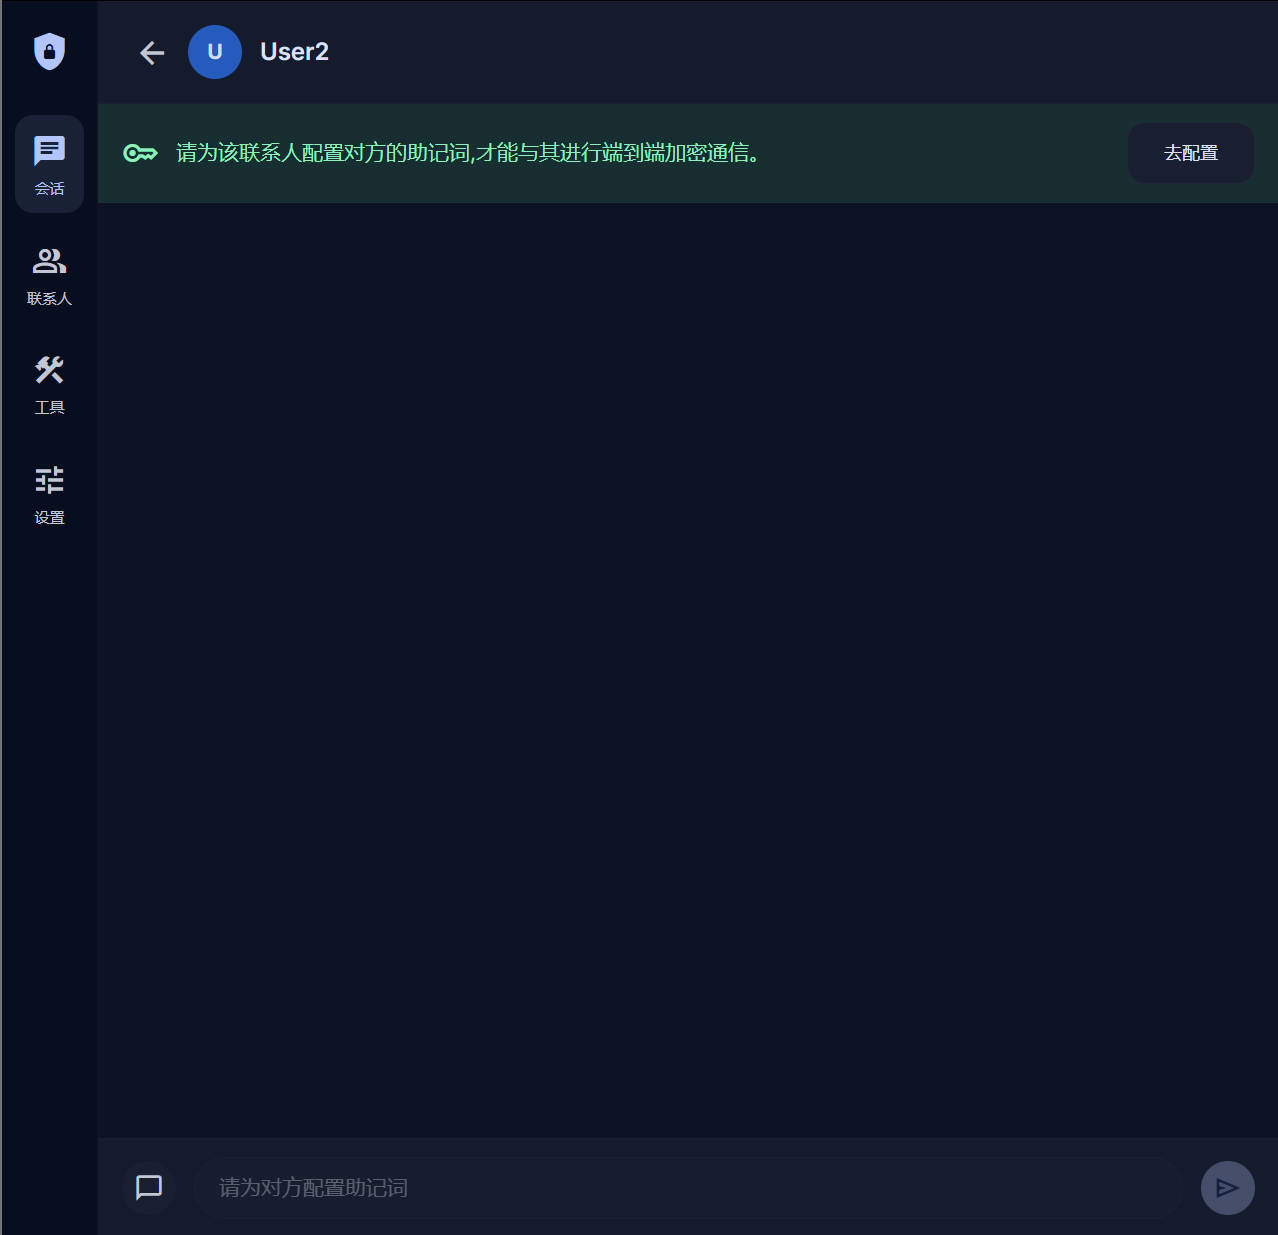
\includegraphics[width=\textwidth]{img/ch5_09_e2ee_banner.jpg}
        \caption{E2EE 状态横幅}
        \label{fig:ch5_e2ee_banner}
    \end{subfigure}
    \hfill
    \begin{subfigure}[b]{0.45\textwidth}
        \centering
        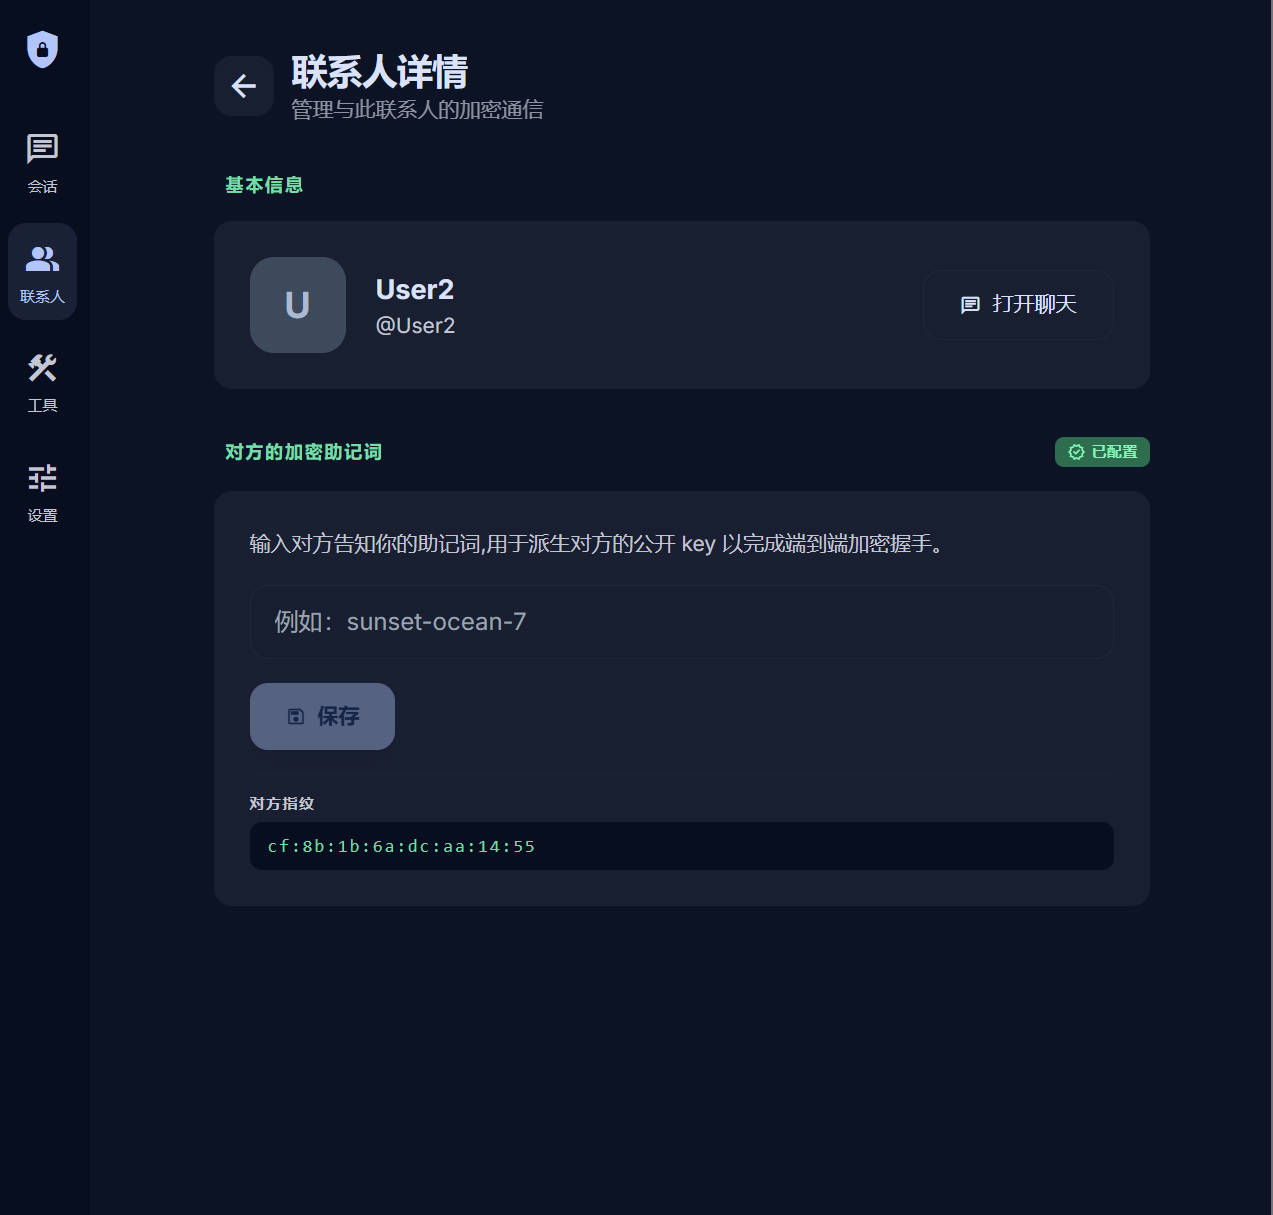
\includegraphics[width=\textwidth]{img/ch5_10_fingerprint.jpg}
        \caption{指纹对比验证}
        \label{fig:ch5_fingerprint}
    \end{subfigure}
    \caption{端到端加密功能}
    \label{fig:ch5_e2ee}
\end{figure}

端到端加密使用固定的黄金测试向量（Golden Test Vectors）进行验证，确保 Android（Kotlin）、Web（TypeScript）和未来可能的服务端（Python）实现之间的互操作性。测试向量包括：已知助记词对应的用户密钥和指纹、已知密钥对和 nonce 对应的加密结果、SealedMessage 序列化格式等。

\subsubsection{隐写嵌入与提取测试}

测试了独立隐写工具页面的嵌入与提取功能，以及双算法切换，测试用例及结果如\cref{tab:test_stego}所示。

\begin{table}[htbp]
    \caption{隐写嵌入与提取测试用例}
    \centering
    \small
    \begin{tabular}{clc}
        \hline
        \textbf{编号} & \textbf{测试内容} & \textbf{结果} \\
        \hline
        T-39 & Pulsar 算法：正常嵌入短文本消息 & 通过 \\
        T-40 & Pulsar 算法：嵌入后正确提取消息 & 通过 \\
        T-41 & SparSamp 算法：正常嵌入短文本消息 & 通过 \\
        T-42 & SparSamp 算法：嵌入后正确提取消息 & 通过 \\
        T-43 & 算法切换：从 Pulsar 切换到 SparSamp & 通过 \\
        T-44 & 模型切换：选择不同预训练模型 & 通过 \\
        T-45 & 超出容量限制时提示错误 & 通过 \\
        T-46 & 使用错误密钥提取（应失败） & 通过 \\
        T-47 & 容量查询接口测试 & 通过 \\
        T-48 & 算法列表查询接口测试 & 通过 \\
        T-49 & SparSamp 状态缓存（第二次请求瞬时返回） & 通过 \\
        \hline
    \end{tabular}
    \label{tab:test_stego}
\end{table}

隐写嵌入和提取页面的测试效果如\cref{fig:ch5_embed_extract}所示。

\begin{figure}[htbp]
    \centering
    \begin{subfigure}[b]{0.45\textwidth}
        \centering
        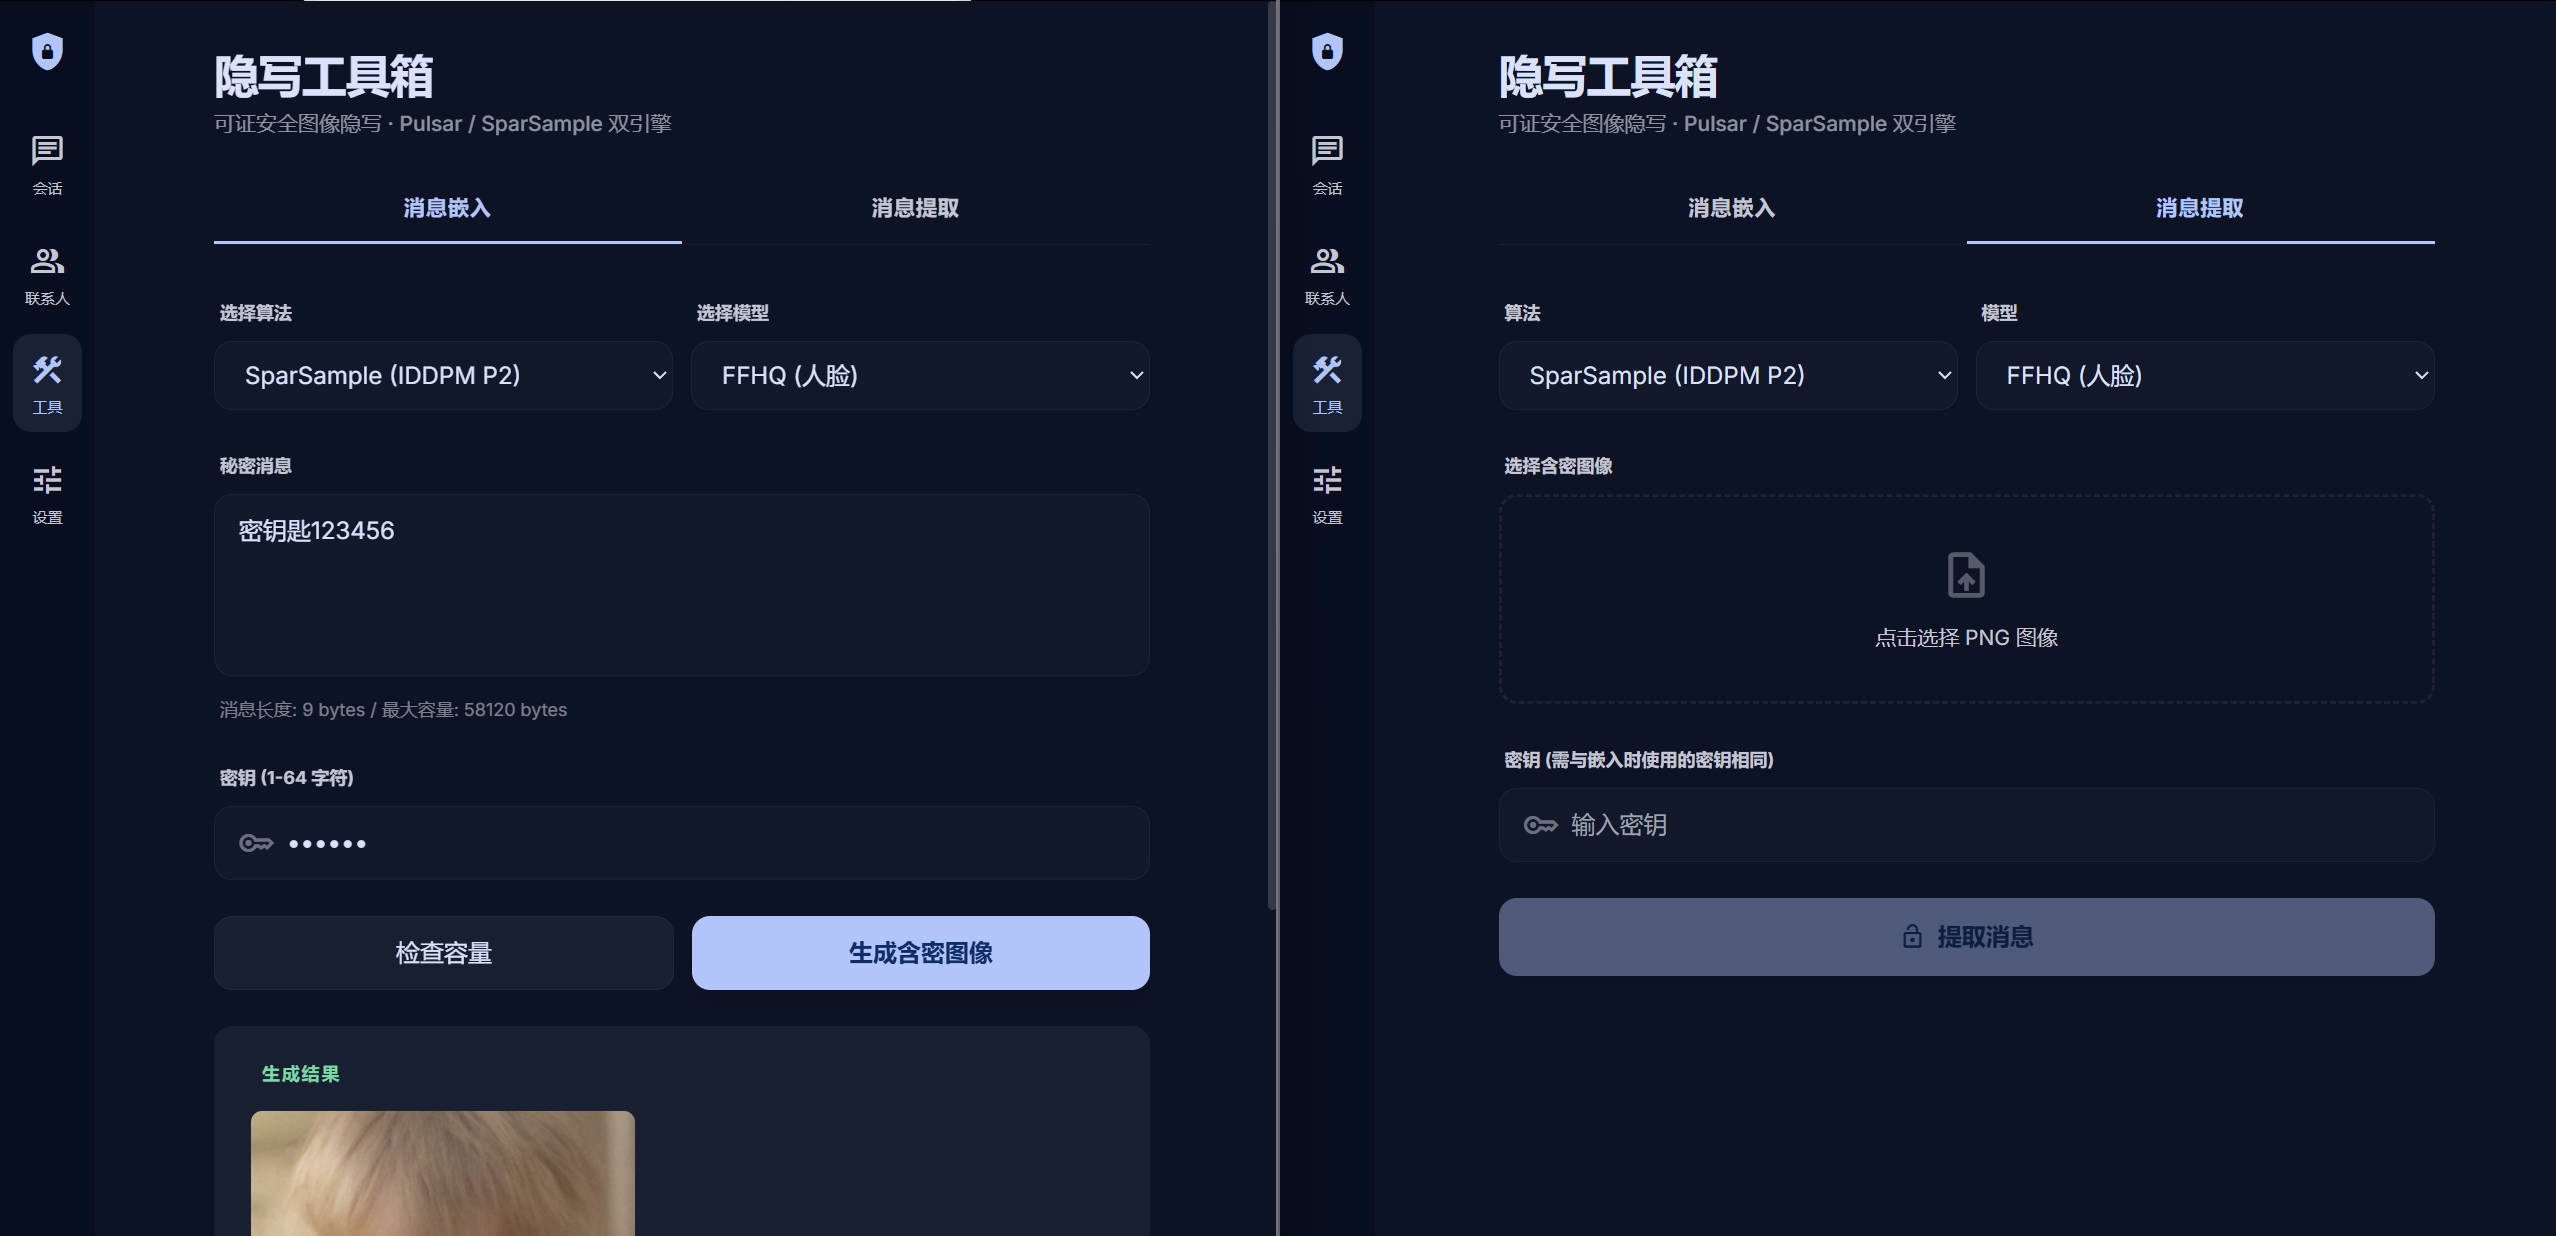
\includegraphics[width=\textwidth]{img/ch5_11_embed.jpg}
        \caption{隐写嵌入页面}
        \label{fig:ch5_embed}
    \end{subfigure}
    \hfill
    \begin{subfigure}[b]{0.45\textwidth}
        \centering
        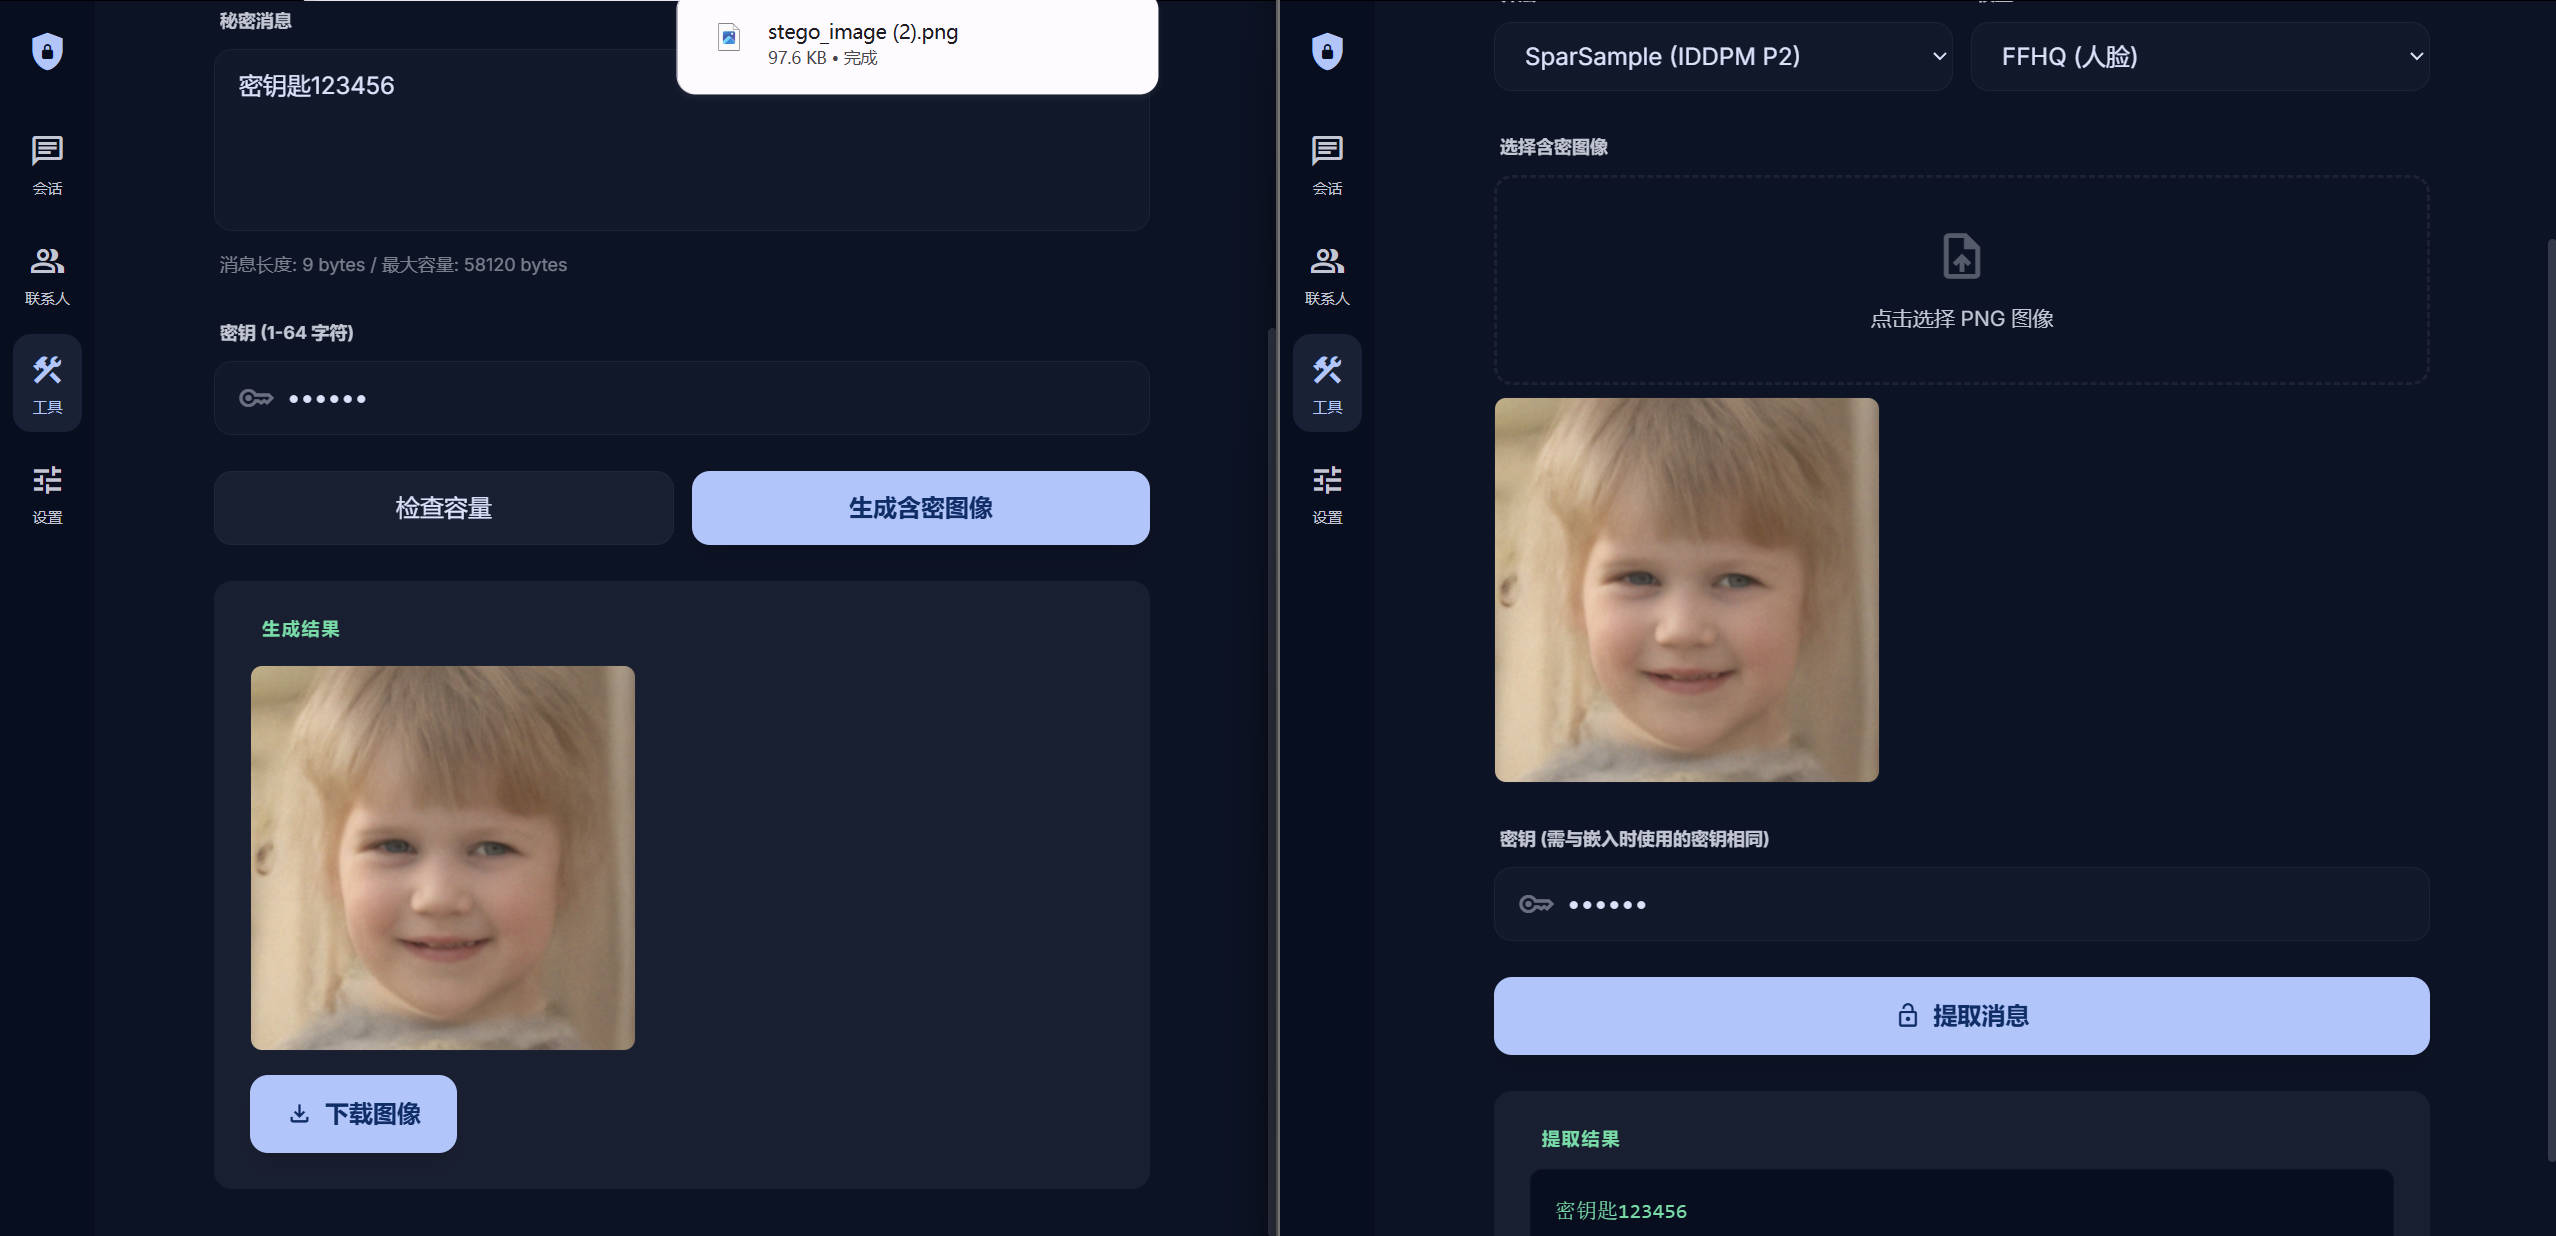
\includegraphics[width=\textwidth]{img/ch5_12_extract.jpg}
        \caption{隐写提取页面}
        \label{fig:ch5_extract}
    \end{subfigure}
    \caption{隐写嵌入与提取功能}
    \label{fig:ch5_embed_extract}
\end{figure}

\subsection{隐写性能分析}

为客观评估两种隐写算法的实际性能，设计了对比实验，使用 5 个随机生成的 24 字节密钥和 3 种不同长度的消息（6、62、150 字节），直接调用算法服务层进行嵌入与提取测试。测试环境为 Ubuntu 22.04 LTS，配备 NVIDIA GPU 和 CUDA 加速。

\subsubsection{算法性能对比}

两种算法的性能对比如\cref{tab:algo_comparison}所示。

\begin{table}[htbp]
    \caption{Pulsar 与 SparSamp 算法性能对比}
    \centering
    \begin{tabular}{lcc}
        \hline
        \textbf{指标} & \textbf{Pulsar (DDIM)} & \textbf{SparSamp (IDDPM P2)} \\
        \hline
        平均嵌入容量 (bytes) & 403 & 58112 \\
        平均嵌入耗时 (s) & 1.9 & 12.4 \\
        平均提取耗时 (s) & 2.4 & 0.03 \\
        提取正确率 & 100\% & 100\% \\
        跨密钥安全 & 是 & 是 \\
        输出图像格式 & 16-bit PNG & 8-bit PNG \\
        图像分辨率 & 256$\times$256 & 256$\times$256 \\
        可证安全性 & 是 & 是 \\
        \hline
    \end{tabular}
    \label{tab:algo_comparison}
\end{table}

表中 Pulsar 的数据基于 CelebA-HQ 256$\times$256 预训练 DDIM 模型，SparSamp 的数据基于 FFHQ 256$\times$256 预训练 IDDPM P2-weighting 模型。

从\cref{tab:algo_comparison}可以看出两种算法在性能特征上存在显著差异：

\begin{enumerate}
    \item \textbf{嵌入容量}：SparSamp 的平均嵌入容量（58,112 字节）远大于 Pulsar（403 字节），约为后者的 144 倍。这是因为 SparSamp 基于稀疏采样机制，通过消息驱动采样在每个像素的量化分布中嵌入消息段，编码空间与图像像素数和消息段长度成正比；而 Pulsar 基于二进制级联纠错码（外码 Reed-Solomon），编码容量受限于图像差异区域的误码率分布和可用纠错码的纠错能力。
    \item \textbf{嵌入耗时}：Pulsar 的嵌入速度（平均 1.9 秒）明显快于 SparSamp（平均 12.4 秒）。Pulsar 仅需执行 50 步 DDIM 采样即可生成含密图像，而 SparSamp 需要执行 1000 步扩散采样（虽然 respaced 为 10 步，但每步计算量较大）。
    \item \textbf{提取耗时}：SparSamp 的提取速度（平均 0.03 秒）远快于 Pulsar（平均 2.4 秒）。SparSamp 的提取过程仅需根据已知的采样结果和 PRNG 状态进行 MRN 更新与候选集合缩小，不涉及模型推理；而 Pulsar 的提取需要重新执行扩散采样以重建编码区域，再进行纠错码解码。
    \item \textbf{正确性与安全性}：两种算法在所有 30 组往返测试中均实现 100\% 提取正确率，跨密钥测试中均无法使用错误密钥提取原始消息，验证了两种算法的正确性和密钥安全性。
\end{enumerate}

两种算法的性能对比如\cref{fig:performance}所示。

\begin{figure}[htbp]
    \centering
    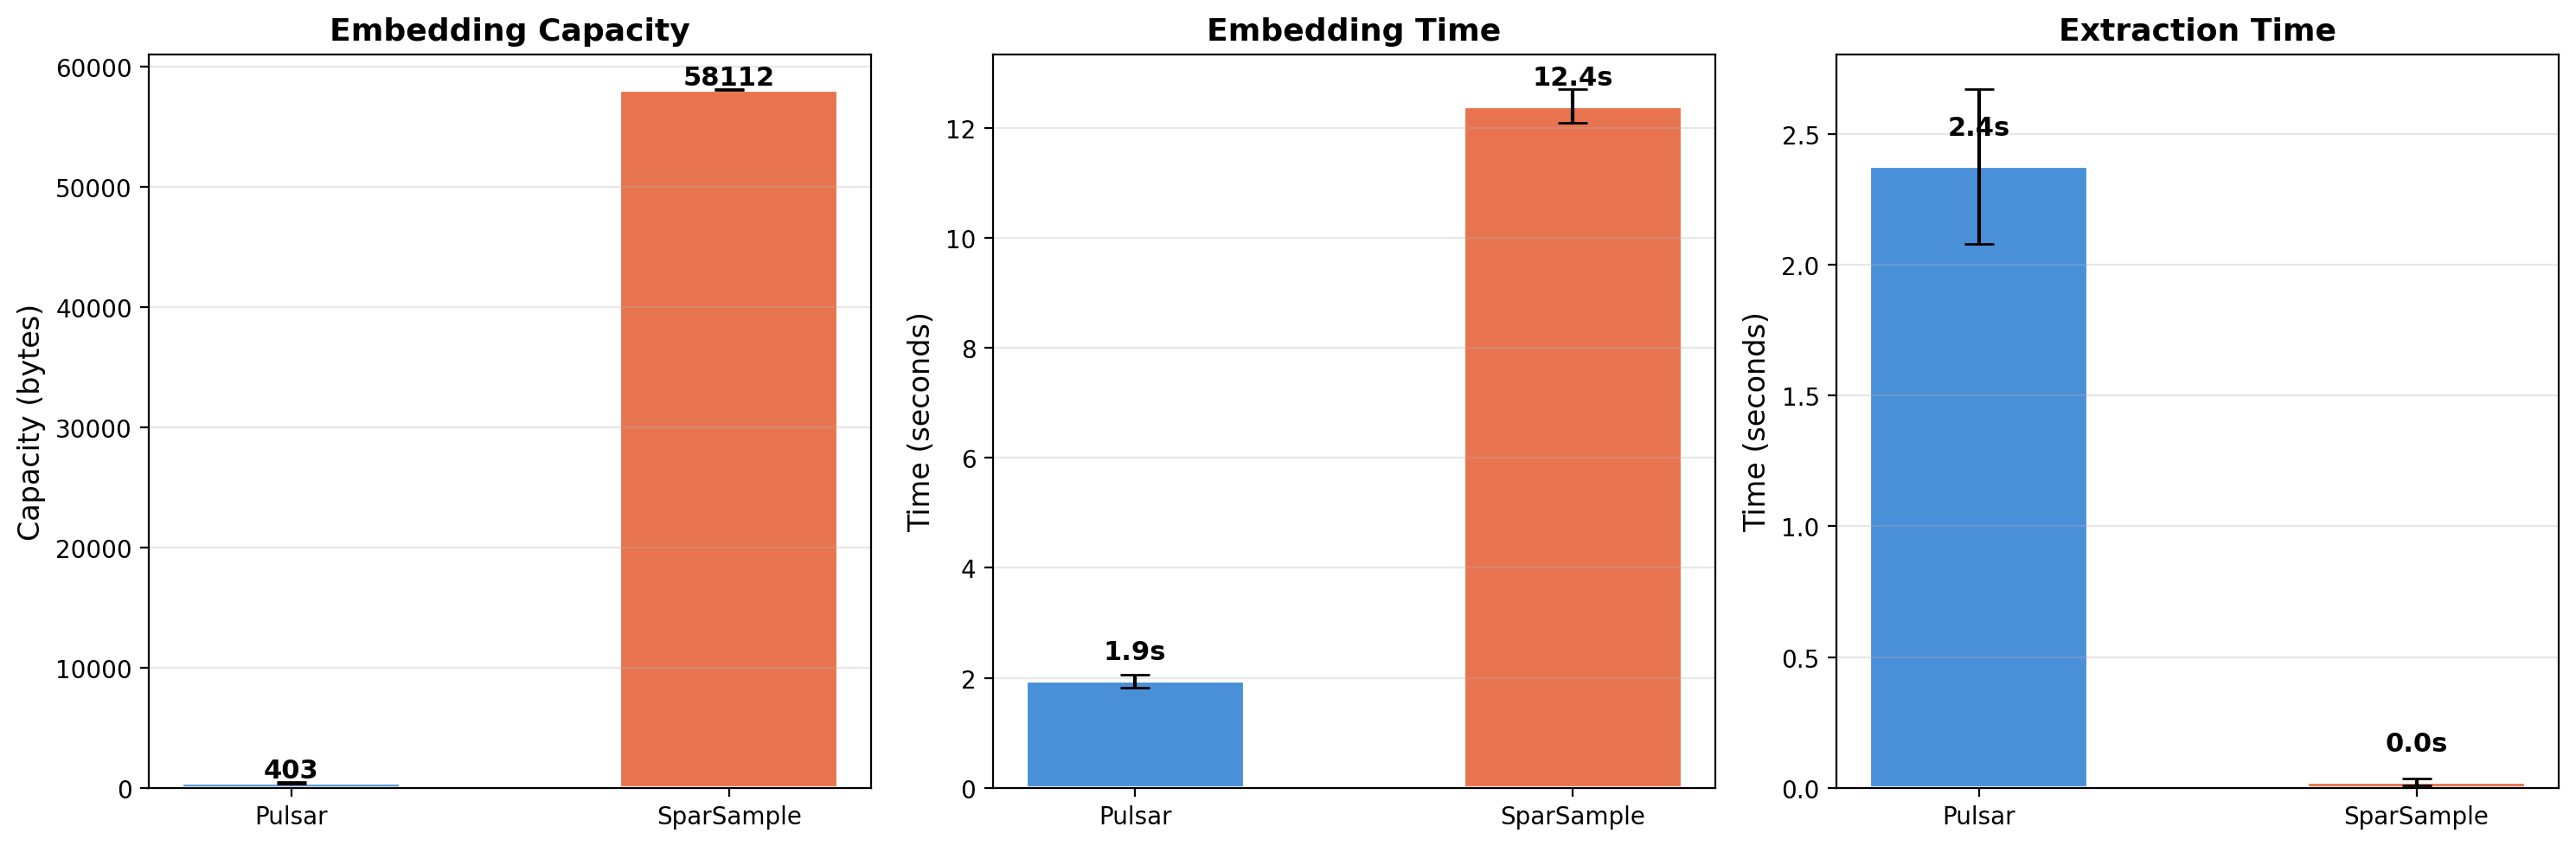
\includegraphics[width=0.85\textwidth]{img/ch5_performance.png}
    \caption{Pulsar 与 SparSamp 性能对比}
    \label{fig:performance}
\end{figure}

综合来看，Pulsar 适合对嵌入速度和提取延迟敏感的应用场景，而 SparSamp 更适合需要大容量隐写的场景。在隐写聊天模式下，由于嵌入的载荷是 E2EE 加密后的 SealedMessage（包含 JSON 信封和 base64url 编码开销），系统将服务器返回的最大容量乘以 0.65 作为安全预算，以容纳加密带来的约 37\% 的数据膨胀。

\subsubsection{安全性分析}

Pulsar 和 SparSamp 两种算法的可证安全性均已在各自的研究工作中得到理论证明。本次实验的跨密钥测试也从实践层面验证了这一特性：使用密钥 A 嵌入的含密图像，使用密钥 B 进行提取时无法恢复原始消息。其安全性保证基于以下共同原理：

\begin{enumerate}
    \item \textbf{分布一致性}：含密图像与正常生成图像都由同一扩散模型生成，差异仅在于采样噪声的来源（PRG vs 真随机数），在分布不可区分的意义下，含密图像与正常生成图像不可区分（KL 散度趋近于 0）。
    \item \textbf{密钥安全性}：不知道密钥的攻击者无法确定编码参数和噪声分配，因此无法从图像中恢复秘密信息。
\end{enumerate}

在端到端加密层面，即使攻击者从隐写图像中提取出了载荷内容，由于载荷是 AES-256-GCM 加密后的密文，没有消息密钥（mkey）也无法解密。消息密钥的派生依赖于双方各自的助记词短语，助记词仅存储在客户端本地，不经过网络传输。

\subsubsection{图像质量}

两种算法生成的图像质量均取决于底层扩散模型的生成能力。由于信息嵌入仅改变了采样路径或最后一步的像素值分布，含密图像的视觉质量与正常生成图像无差异。使用 256$\times$256 分辨率的预训练模型时，生成的图像具有较高的真实感。

为量化评估含密图像的质量损失，分别计算了含密图像与对应原始扩散模型生成图像之间的峰值信噪比（PSNR）、结构相似性（SSIM）以及弗雷歇起始距离（FID），结果如\cref{tab:image_quality}所示。其中 PSNR 和 SSIM 基于 20 组含密--原图配对计算均值，FID 基于 20 张含密图像与 20 张原始生成图像的分布距离计算。实验在 NVIDIA RTX 3060 Laptop GPU 上完成，总耗时约 47 分钟。

\begin{table}[htbp]
    \caption{含密图像与原始生成图像的质量对比}
    \centering
    \begin{tabular}{lccc}
        \hline
        \textbf{算法 / 模型} & \textbf{PSNR (dB)} & \textbf{SSIM} & \textbf{FID} \\
        \hline
        Pulsar / CelebA-HQ DDIM & 60.04 & 1.0000 & 0.06 \\
        SparSamp / FFHQ IDDPM P2 & 42.77 & 0.9988 & 1.76 \\
        \hline
    \end{tabular}
    \label{tab:image_quality}
\end{table}

\begin{figure}[htbp]
    \centering
    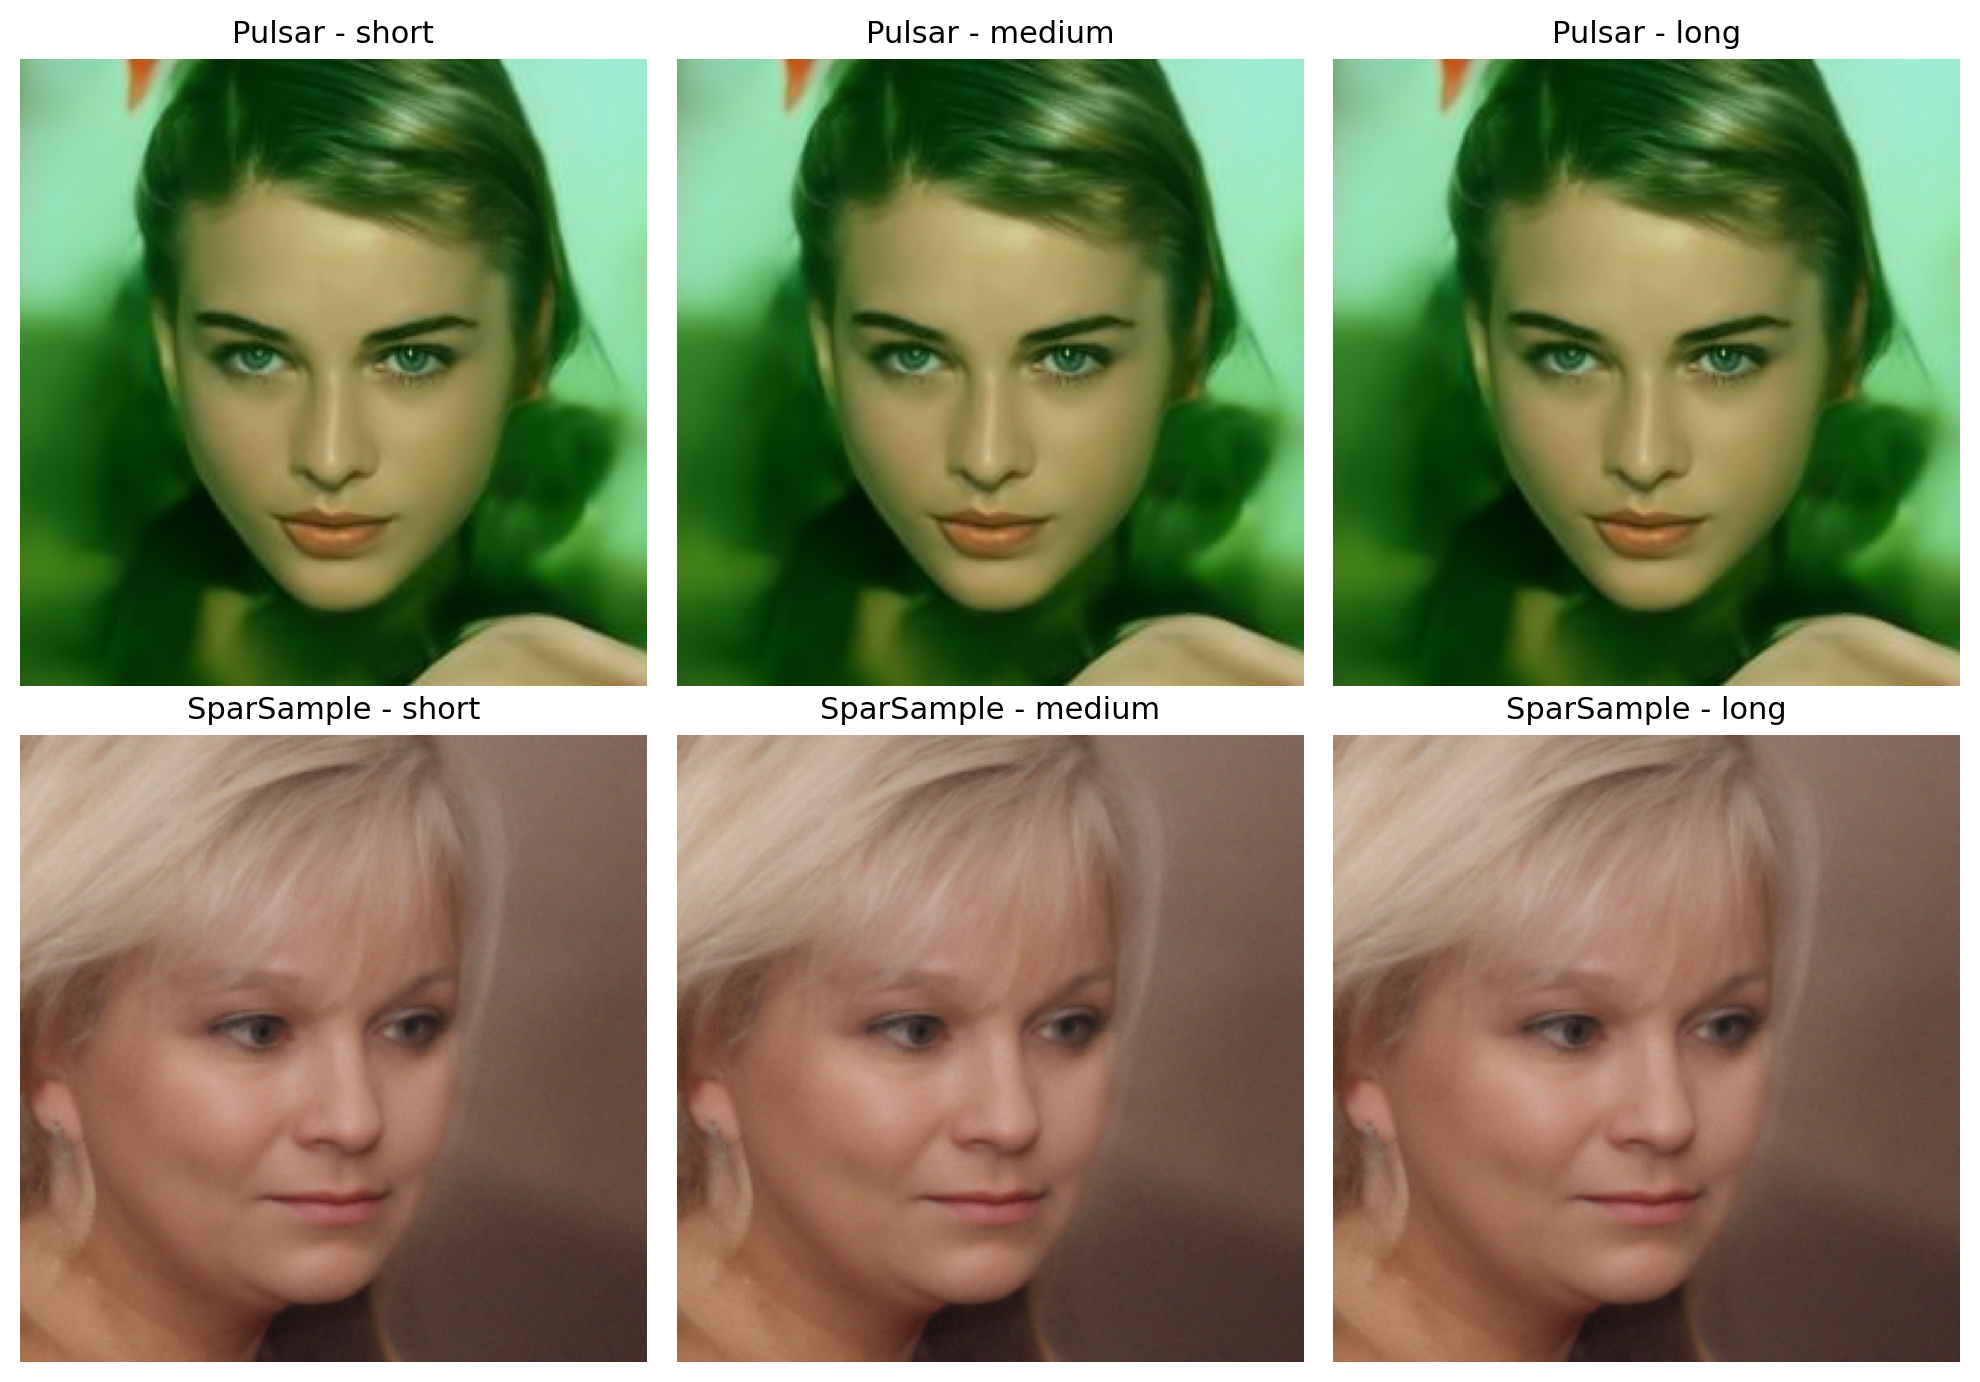
\includegraphics[width=0.85\textwidth]{img/ch5_sample_compare.png}
    \caption{隐写样本对比}
    \label{fig:sample_compare}
\end{figure}

在实际聊天场景中使用隐写模式的效果如\cref{fig:ch5_stego_chat}所示。发送方在隐写模式下输入文本消息后，系统自动将消息嵌入到扩散模型生成的含密图像中并发送给接收方；接收方点击图像即可提取出原始文本消息，整个过程对用户透明。

\begin{figure}[htbp]
    \centering
    \begin{subfigure}[b]{0.45\textwidth}
        \centering
        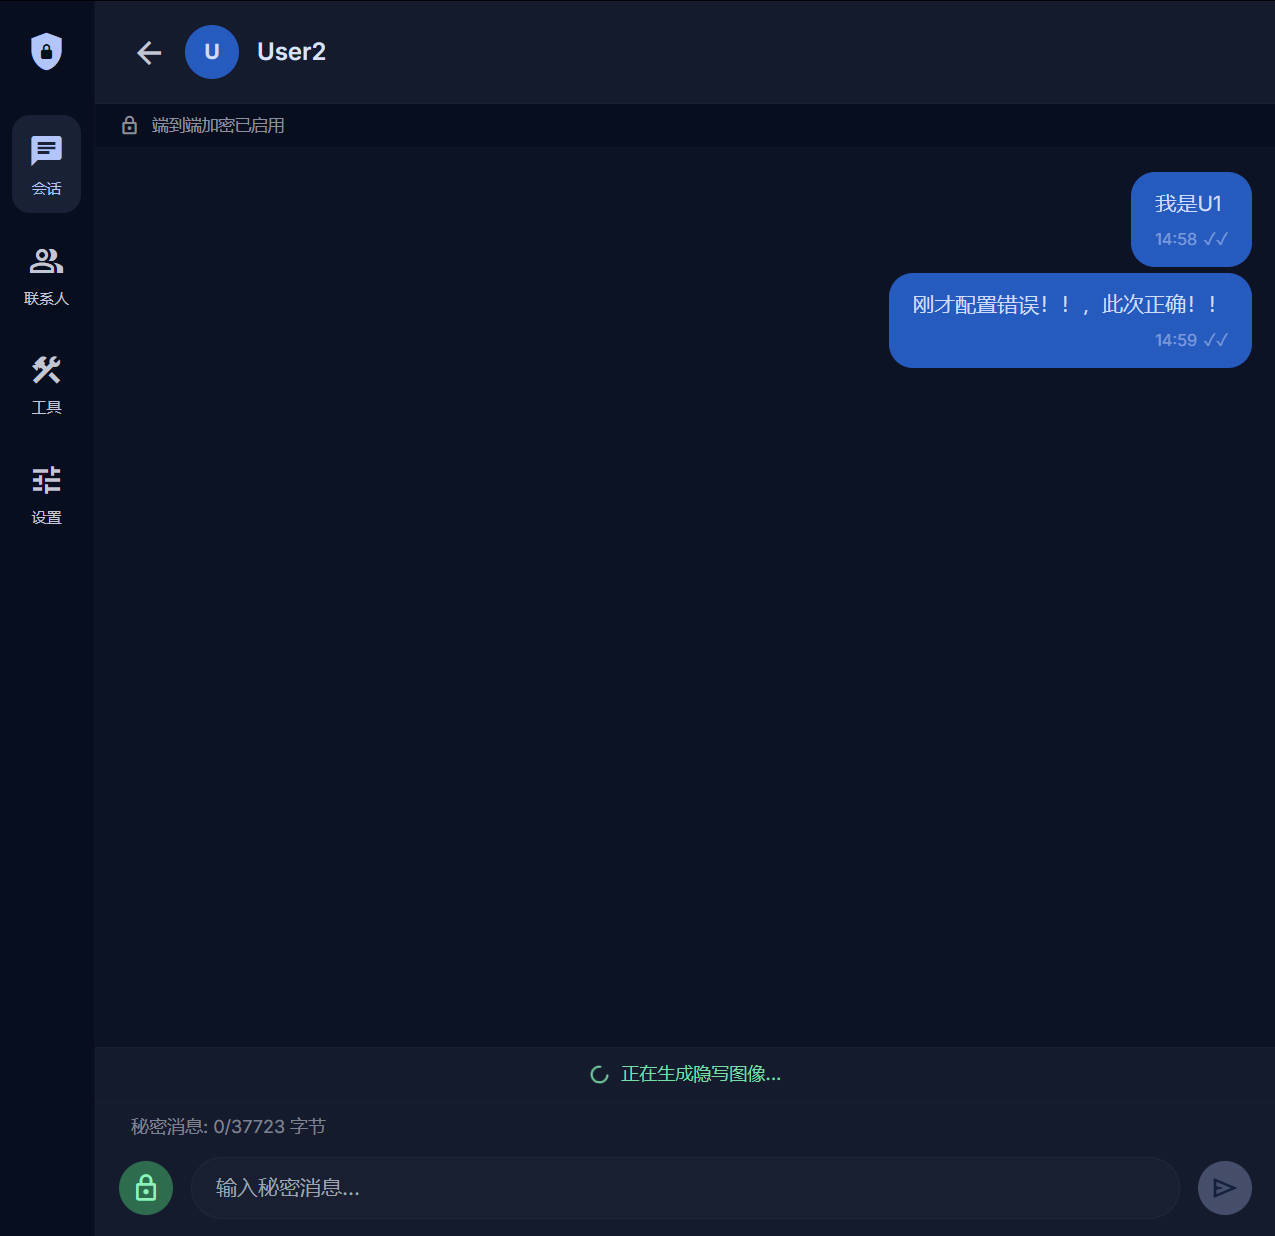
\includegraphics[width=\textwidth]{img/ch5_13_stego_chat.jpg}
        \caption{Web 端隐写聊天}
        \label{fig:ch5_stego_web}
    \end{subfigure}
    \hfill
    \begin{subfigure}[b]{0.45\textwidth}
        \centering
        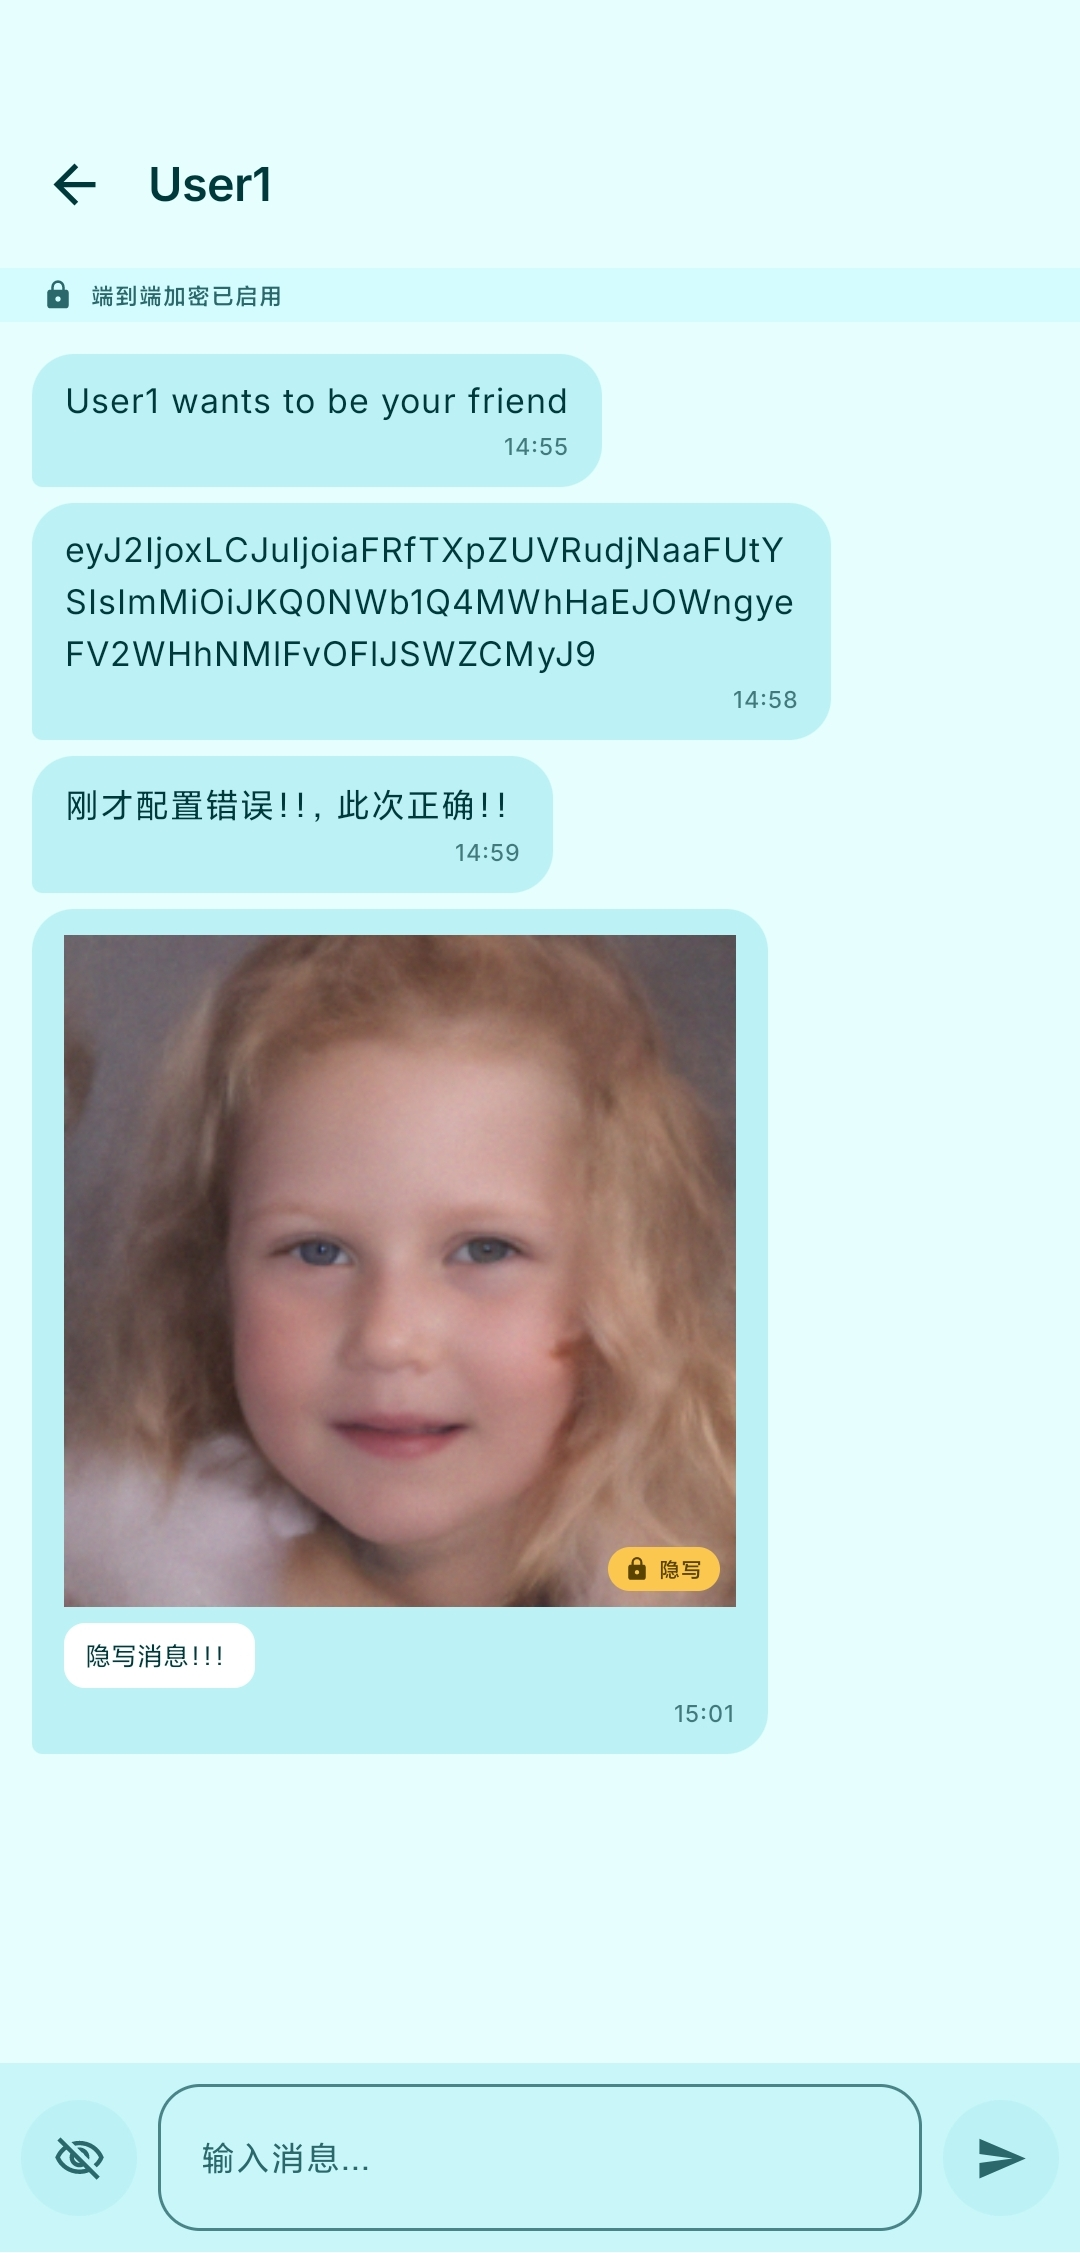
\includegraphics[height=6cm]{img/ch5_13_stego_chat_phone.jpg}
        \caption{Android 端隐写聊天}
        \label{fig:ch5_stego_android}
    \end{subfigure}
    \caption{隐写模式聊天效果}
    \label{fig:ch5_stego_chat}
\end{figure}

\subsection{跨平台兼容性测试}

系统设计的一个重要目标是支持跨平台通信。测试了 Android 客户端与 Web 客户端之间的互操作性，结果如\cref{tab:test_cross}所示。

\begin{table}[htbp]
    \caption{跨平台兼容性测试}
    \centering
    \begin{tabular}{clc}
        \hline
        \textbf{编号} & \textbf{测试场景} & \textbf{结果} \\
        \hline
        T-50 & Android 发送普通消息 $\to$ Web 接收 & 通过 \\
        T-51 & Web 发送普通消息 $\to$ Android 接收 & 通过 \\
        T-52 & Android 发送加密消息 $\to$ Web 解密 & 通过 \\
        T-53 & Web 发送加密消息 $\to$ Android 解密 & 通过 \\
        T-54 & Android 发送隐写消息 $\to$ Web 提取 & 通过 \\
        T-55 & Web 发送隐写消息 $\to$ Android 提取 & 通过 \\
        T-56 & Android 发送好友请求 $\to$ Web 处理 & 通过 \\
        T-57 & Web 发送好友请求 $\to$ Android 处理 & 通过 \\
        T-58 & 单端登录：Android 登录后 Web 被踢出 & 通过 \\
        T-59 & 单端登录：Web 登录后 Android 被踢出 & 通过 \\
        T-60 & 消息状态回执跨平台同步 & 通过 \\
        \hline
    \end{tabular}
    \label{tab:test_cross}
\end{table}

单端登录机制的测试效果如\cref{fig:ch5_single_login}所示，当用户在 Android 端登录后，Web 端自动弹出提示并跳转至登录页面，验证了单端登录策略的有效性。

\begin{figure}[htbp]
    \centering
    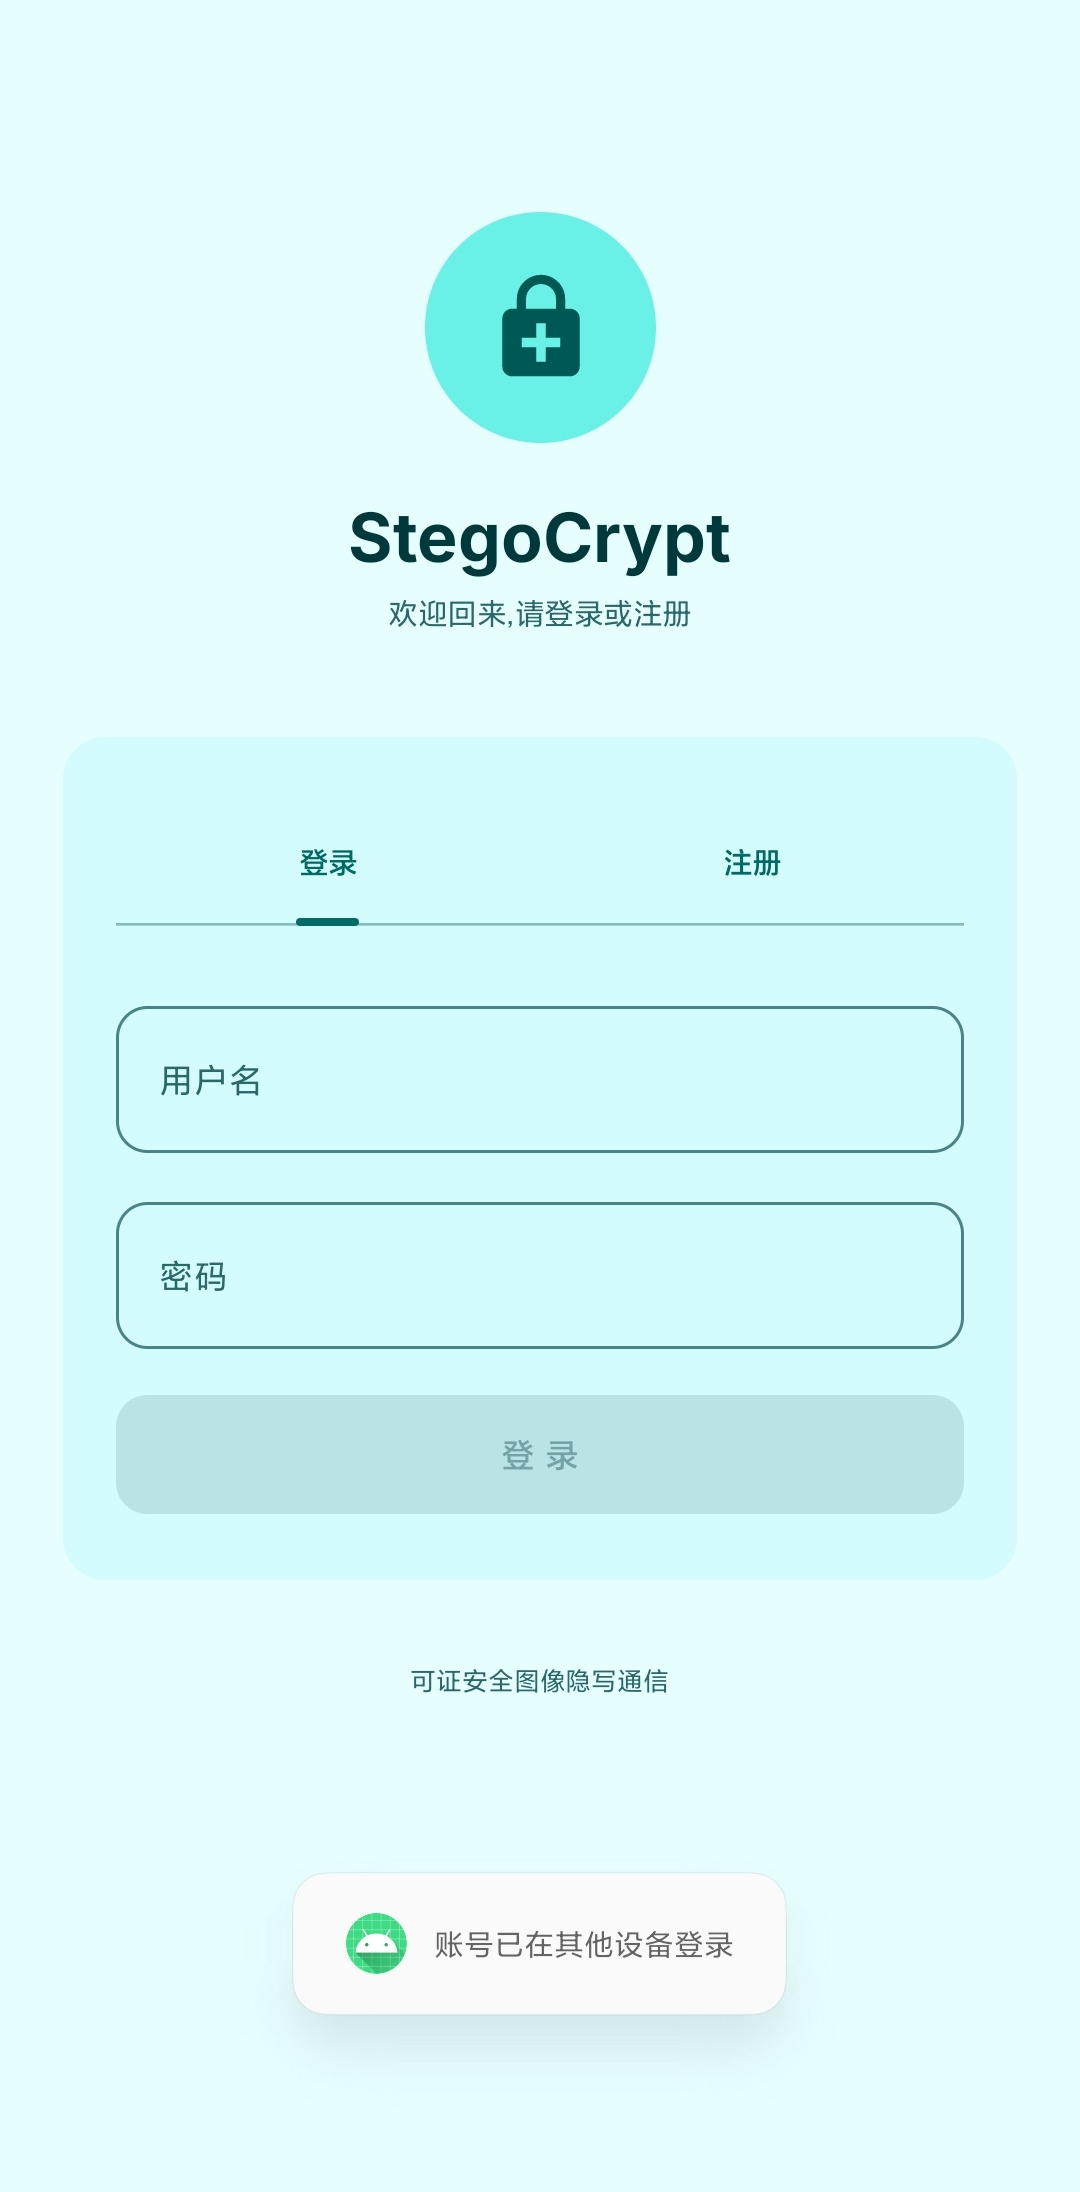
\includegraphics[width=0.55\textwidth]{img/ch5_single_login.jpg}
    \caption{单端登录效果}
    \label{fig:ch5_single_login}
\end{figure}

测试结果表明，Android 客户端和 Web 客户端之间能够正常互相发送普通消息和隐写消息，端到端加密的跨平台加解密正确，好友管理、消息状态管理和单端登录功能跨平台工作正常。SealedMessage 的 JSON 信封格式和 base64url 编码在两个平台间完全兼容。

\subsection{本章小结}

本章从功能测试、隐写性能分析和跨平台兼容性三个维度对系统进行了全面测试。功能测试覆盖了用户管理、好友管理、消息生命周期、端到端加密和隐写操作等核心功能，共计 60 个测试用例全部通过。隐写性能分析验证了双算法在安全性和图像质量方面的表现，以及端到端加密对隐写载荷的双重保护。跨平台兼容性测试确认了 Android 和 Web 客户端之间的完整互操作性，包括加密消息、隐写消息和消息状态回执的跨平台同步。测试结果表明系统功能完整、运行稳定。
